\documentclass{article}

  % packages
    % basic stuff for rendering math
    \usepackage[letterpaper, top=1in, bottom=1in, left=1in, right=1in]{geometry}
    \usepackage[utf8]{inputenc}
    \usepackage[english]{babel}
    \usepackage{amsmath} 
    \usepackage{amssymb}
    % \usepackage{amsthm}

    % extra math symbols and utilities
    \usepackage{mathtools}        % for extra stuff like \coloneqq
    \usepackage{mathrsfs}         % for extra stuff like \mathsrc{}
    \usepackage{centernot}        % for the centernot arrow 
    \usepackage{bm}               % for better boldsymbol/mathbf 
    \usepackage{enumitem}         % better control over enumerate, itemize
    \usepackage{hyperref}         % for hypertext linking
    \usepackage{fancyvrb}          % for better verbatim environments
    \usepackage{newverbs}         % for texttt{}
    \usepackage{xcolor}           % for colored text 
    \usepackage{listings}         % to include code
    \usepackage{lstautogobble}    % helper package for code
    \usepackage{parcolumns}       % for side by side columns for two column code
    \usepackage{algorithm, algpseudocode}
    

    % page layout
    \usepackage{fancyhdr}         % for headers and footers 
    \usepackage{lastpage}         % to include last page number in footer 
    \usepackage{parskip}          % for no indentation and space between paragraphs    
    \usepackage[T1]{fontenc}      % to include \textbackslash
    \usepackage{footnote}
    \usepackage{etoolbox}

    % for custom environments
    \usepackage{tcolorbox}        % for better colored boxes in custom environments
    \tcbuselibrary{breakable}     % to allow tcolorboxes to break across pages

    % figures
    \usepackage{pgfplots}
    \pgfplotsset{compat=1.18}
    \usepackage{float}            % for [H] figure placement
    \usepackage{tikz}
    \usepackage{tikz-cd}
    \usepackage{circuitikz}
    \usetikzlibrary{arrows}
    \usetikzlibrary{positioning}
    \usetikzlibrary{calc}
    \usepackage{graphicx}
    \usepackage{caption} 
    \usepackage{subcaption}
    \captionsetup{font=small}

    % for tabular stuff 
    \usepackage{dcolumn}

    \usepackage[nottoc]{tocbibind}
    \pdfsuppresswarningpagegroup=1
    \hfuzz=5.002pt                % ignore overfull hbox badness warnings below this limit

  % New and replaced operators
    \DeclareMathOperator{\Tr}{Tr}
    \DeclareMathOperator{\Sym}{Sym}
    \DeclareMathOperator{\Span}{span}
    \DeclareMathOperator{\prox}{prox}
    \DeclareMathOperator{\std}{std}
    \DeclareMathOperator{\Cov}{Cov}
    \DeclareMathOperator{\Var}{Var}
    \DeclareMathOperator{\Corr}{Corr}
    \DeclareMathOperator{\pos}{pos}
    \DeclareMathOperator*{\argmin}{\arg\!\min}
    \DeclareMathOperator*{\argmax}{\arg\!\max}
    \newcommand{\qed}{\hfill$\blacksquare$}     % I like QED squares to be black

  % Custom Environments
    \newtcolorbox[auto counter, number within=section]{question}[1][]
    {
      colframe = orange!25,
      colback  = orange!10,
      coltitle = orange!20!black,  
      breakable, 
      title = \textbf{Question \thetcbcounter ~(#1)}
    }

    \newtcolorbox[auto counter, number within=section]{exercise}[1][]
    {
      colframe = teal!25,
      colback  = teal!10,
      coltitle = teal!20!black,  
      breakable, 
      title = \textbf{Exercise \thetcbcounter ~(#1)}
    }
    \newtcolorbox[auto counter, number within=section]{solution}[1][]
    {
      colframe = violet!25,
      colback  = violet!10,
      coltitle = violet!20!black,  
      breakable, 
      title = \textbf{Solution \thetcbcounter}
    }
    \newtcolorbox[auto counter, number within=section]{lemma}[1][]
    {
      colframe = red!25,
      colback  = red!10,
      coltitle = red!20!black,  
      breakable, 
      title = \textbf{Lemma \thetcbcounter ~(#1)}
    }
    \newtcolorbox[auto counter, number within=section]{theorem}[1][]
    {
      colframe = red!25,
      colback  = red!10,
      coltitle = red!20!black,  
      breakable, 
      title = \textbf{Theorem \thetcbcounter ~(#1)}
    } 
    \newtcolorbox[auto counter, number within=section]{proposition}[1][]
    {
      colframe = red!25,
      colback  = red!10,
      coltitle = red!20!black,  
      breakable, 
      title = \textbf{Proposition \thetcbcounter ~(#1)}
    } 
    \newtcolorbox[auto counter, number within=section]{corollary}[1][]
    {
      colframe = red!25,
      colback  = red!10,
      coltitle = red!20!black,  
      breakable, 
      title = \textbf{Corollary \thetcbcounter ~(#1)}
    } 
    \newtcolorbox[auto counter, number within=section]{proof}[1][]
    {
      colframe = orange!25,
      colback  = orange!10,
      coltitle = orange!20!black,  
      breakable, 
      title = \textbf{Proof. }
    } 
    \newtcolorbox[auto counter, number within=section]{definition}[1][]
    {
      colframe = yellow!25,
      colback  = yellow!10,
      coltitle = yellow!20!black,  
      breakable, 
      title = \textbf{Definition \thetcbcounter ~(#1)}
    } 
    \newtcolorbox[auto counter, number within=section]{example}[1][]
    {
      colframe = blue!25,
      colback  = blue!10,
      coltitle = blue!20!black,  
      breakable, 
      title = \textbf{Example \thetcbcounter ~(#1)}
    } 
    \newtcolorbox[auto counter, number within=section]{code}[1][]
    {
      colframe = green!25,
      colback  = green!10,
      coltitle = green!20!black,  
      breakable, 
      title = \textbf{Code \thetcbcounter ~(#1)}
    } 

    \BeforeBeginEnvironment{example}{\savenotes}
    \AfterEndEnvironment{example}{\spewnotes}
    \BeforeBeginEnvironment{lemma}{\savenotes}
    \AfterEndEnvironment{lemma}{\spewnotes}
    \BeforeBeginEnvironment{theorem}{\savenotes}
    \AfterEndEnvironment{theorem}{\spewnotes}
    \BeforeBeginEnvironment{corollary}{\savenotes}
    \AfterEndEnvironment{corollary}{\spewnotes}
    \BeforeBeginEnvironment{proposition}{\savenotes}
    \AfterEndEnvironment{proposition}{\spewnotes}
    \BeforeBeginEnvironment{definition}{\savenotes}
    \AfterEndEnvironment{definition}{\spewnotes}
    \BeforeBeginEnvironment{exercise}{\savenotes}
    \AfterEndEnvironment{exercise}{\spewnotes}
    \BeforeBeginEnvironment{proof}{\savenotes}
    \AfterEndEnvironment{proof}{\spewnotes}
    \BeforeBeginEnvironment{solution}{\savenotes}
    \AfterEndEnvironment{solution}{\spewnotes}
    \BeforeBeginEnvironment{question}{\savenotes}
    \AfterEndEnvironment{question}{\spewnotes}
    \BeforeBeginEnvironment{code}{\savenotes}
    \AfterEndEnvironment{code}{\spewnotes}

    \definecolor{dkgreen}{rgb}{0,0.6,0}
    \definecolor{gray}{rgb}{0.5,0.5,0.5}
    \definecolor{mauve}{rgb}{0.58,0,0.82}
    \definecolor{lightgray}{gray}{0.93}

    % default options for listings (for code)
    \lstset{
      autogobble,
      frame=ltbr,
      language=C,                           % the language of the code
      aboveskip=3mm,
      belowskip=3mm,
      showstringspaces=false,
      columns=fullflexible,
      keepspaces=true,
      basicstyle={\small\ttfamily},
      numbers=left,
      firstnumber=1,                        % start line number at 1
      numberstyle=\tiny\color{gray},
      keywordstyle=\color{blue},
      commentstyle=\color{dkgreen},
      stringstyle=\color{mauve},
      backgroundcolor=\color{lightgray}, 
      breaklines=true,                      % break lines
      breakatwhitespace=true,
      tabsize=3, 
      xleftmargin=2em, 
      framexleftmargin=1.5em, 
      stepnumber=1
    }

  % Page style
    \pagestyle{fancy}
    \fancyhead[L]{Sampling, Optimization, and Intergration}
    \fancyhead[C]{Muchang Bahng}
    \fancyhead[R]{Spring 2024} 
    \fancyfoot[C]{\thepage / \pageref{LastPage}}
    \renewcommand{\footrulewidth}{0.4pt}          % the footer line should be 0.4pt wide
    \renewcommand{\thispagestyle}[1]{}  % needed to include headers in title page

\begin{document}

\title{Sampling, Optimization, and Integration}
\author{Muchang Bahng}
\date{November 2022}

\maketitle
\tableofcontents
\pagebreak

This covers computability theory, complexity theory, and automata theory. 
Alphabet. Boolean logic


\section{Gradient Descent} 

  Note that gradient computation is generally very expensive and not scalable as $n$ gets high. Given a dataset $\mathcal{D} = \{d_i\}_i$ of $D$ points, our posterior is of the form $p(\theta \mid \mathcal{D}) \propto p(\mathcal{D} \mid \theta) \, p(\theta)$ and so 
  \begin{equation}
    \nabla_\theta \log p(\theta \mid \mathcal{D}) = \nabla_\theta \log{p(\theta)} + \nabla_\theta \log{p(\mathcal{D} \mid \theta)} = \nabla_\theta \log{p(\theta)} + \sum_i \nabla_\theta \log{p(d_i \mid \theta)}
  \end{equation}

  We can approximate this gradient by taking a minibatch of $\mathcal{D}$. Let us take a minibatch of $m$ samples $M_m (\mathcal{D})$ without replacement, where $m << D$. Then, our approximation of the gradient of the log likelihood is 

  \begin{equation}
    \nabla_\theta \log{p(\mathcal{D} \mid \theta)} \approx \nabla_\theta \log{p (M_m (\mathcal{D}) \mid \theta)} \coloneqq \frac{D}{m} \sum_{d \in M_m(\mathcal{D})} \nabla_\theta \log{p(d \mid \theta)}
  \end{equation}

  and thus our noisy gradient approximation of the gradient of the log posterior is 

  \begin{equation}
    \nabla_\theta \log{p(\theta \mid \mathcal{D})} \approx \nabla_\theta \log{p(\theta \mid M_m(\mathcal{D}))} \coloneqq \nabla_\theta \log{p(\theta)} + \nabla_\theta \log{p (M_m (\mathcal{D}) \mid \theta)}
  \end{equation}

\subsection{SGD} 

  The classical gradient ascent algorithm simply optimizes a concave function, or if $f$ is multimodal, finds a local maxima. When we use the entire $\mathcal{D}$ to compute the gradient, we call this a \textit{batch gradient descent}, and if the minibatch estimate of the gradient is used, then this is called \textit{stochastic gradient descent}. Ideally, we would want to have a variable step size $h(t)$ so that $h \rightarrow 0$ as $t \rightarrow + \infty$. 

  \begin{algorithm}
    \caption{Stochastic Gradient Ascent}\label{alg:sgd}
    \begin{algorithmic}

    \Require Initial $\boldsymbol{\theta}_0$, Stepsize function $h(t)$, Minibatch size $m$

    \For{$t = 0$ to $T$ until convergence,}
        \State $\hat{g}(\theta_t) \gets \nabla_\theta \log{p(\theta_t \mid M_m(\mathcal{D}))}$
        \State $\theta_{t+1} \gets \theta_t + h(t) \cdot \hat{g}(\theta_t)$
    \EndFor

    \end{algorithmic}
  \end{algorithm}

  SGD with momentum. 

\subsection{RMSProp} 

\subsection{Adam} 

\subsection{Adagrad}

\subsection{Sparsity-Inducing SGD} 

  We can do SGD with clipping. 

\subsection{Block Coordinate Descent} 

\subsection{Proximal Gradient Descent}

  \subsubsection{Subdifferentials}

    \begin{definition}[Convex Function]
      A function $f: U \subset \mathbb{R}^n \rightarrow \mathbb{R}$ defined on a convex set $U$ is convex if and only if for any $\mathbf{x}, \mathbf{y} \in U$
      \begin{equation}
        f \big(\lambda \mathbf{x} + (1 - \lambda) \mathbf{y} \big) \leq \lambda f(\mathbf{x}) + (1 - \lambda) f(\mathbf{y})
      \end{equation}
      Now if $f$ is differentiable, then convexity is equivalent to 
      \begin{equation}
        f(x) \geq f(y) + \nabla f(y)^T \cdot (x - y)
      \end{equation}
      for all $x, y \in U$. That is, its local linear approximation always underestimates $f$. 
    \end{definition}

    It is well known that the mean square error of a linear map is convex. However, when we impose the L1 penalty, the loss function is now not differentiable at $\mathbf{0}$. Therefore, we must introduce the notion of a subgradient. 

    \begin{definition}[Subgradient]
      The subgradient of a convex function $f: U \subset \mathbb{R}^n \rightarrow \mathbb{R}$ is any linear map $\mathbf{A} (x): \mathbb{R}^n \rightarrow \mathbb{R}$ such that 
      \begin{equation}
        f(\mathbf{y}) \geq f(\mathbf{x}) + \mathbf{A}(\mathbf{x}) (\mathbf{y} - \mathbf{x})
      \end{equation}
      for any $\mathbf{y} \in U$. The set of all subgradients at $\mathbf{x}$ is called the \textbf{subdifferential} defined 
      \begin{equation}
        \partial f (\mathbf{x}) = \{ \mathbf{A} \in \mathbb{R}^n \mid \mathbf{A} \text{ is a subgradient of } f \text{ at } \mathbf{x} \}
      \end{equation}
    \end{definition}

    The subgradient also acts as a linear approximation of $f$, but now at nondifferentiable points of convex functions, we have a set of linear approximations. It is clear that the subgradient at a differentiable point is uniquely the gradient ($\partial f(\mathbf{x}) = \{ \nabla f(\mathbf{x})$), but for places like the absolute value, we can have infinite linear approximations. 
    \begin{center}
      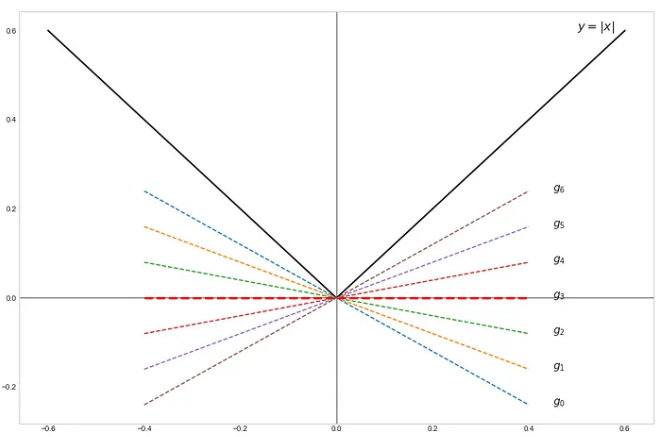
\includegraphics[scale=0.4]{img/subgradient_of_abs.png}
    \end{center}
    Given the subdifferential, thus the optimality condition for any convex $\mathbf{f}$ (differentiable or not) is
    \begin{equation}
      f(\mathbf{x}^\ast) = \min_{\mathbf{x}} f(\mathbf{x}) \iff \mathbf{0} \in \partial f(\mathbf{x}^\ast)
    \end{equation}
    known as the subgradient optimality condition, which clearly implies 
    \begin{equation}
      f(\mathbf{y}) \geq f(\mathbf{x}^\ast) + \mathbf{0}^T (\mathbf{y} - \mathbf{x}^\ast) = f(\mathbf{x}^\ast)
    \end{equation}

    \begin{example}
      The subdifferential of the absolute value function $f(x) = |x|$ at any given $x$ is 
      \begin{equation}
        \partial f(x) = \begin{cases} 1 & \text{ if } x > 0 \\ [-1, 1] & \text{ if } x = 0 \\ -1 & \text{ if } x < 0 \end{cases}
      \end{equation}
    \end{example}

  \subsubsection{Proximal Operators and Soft Thresholding}

    \begin{definition}[Proximal Operator]
      Given a lower semicontinuous convex function $f$ mapping from Hilbert space $X$ to $[-\infty, +\infty]$, its \textbf{proximal operator} associated with a point $u$ is defined 
      \begin{equation}
        \prox_{f, \tau} (u) = \argmin_{x} \bigg( f(x) + \frac{1}{2\tau} ||x - u||^2 \bigg)
      \end{equation}
      where $\tau > 0$ is a parameter that scales the quadratic term. This is basically the point that minimizes the sum of $f(x)$ and the square of the Euclidean distance between $x$ and $u$, scaled by $1/2\tau$. 
    \end{definition}

    Now given the loss function $L (\boldsymbol{\theta}) = L_{\mathrm{obj}} (\boldsymbol{\theta}) + L_{\mathrm{reg}} (\boldsymbol{\theta})$, we want to compute the proximal operator on the regularization loss and update that with the gradient of the smooth objective loss. 
    \begin{equation}
      \boldsymbol{\theta}^{(k+1)} = \prox_{L_{\mathrm{reg}}, \tau} \big[ \boldsymbol{\theta}^{(k)} - \tau \nabla L_{\mathrm{obj}} (\boldsymbol{\theta}^{(k)}) \big]
    \end{equation}
    Let's compute the proximal operator of the L1 loss $h(\boldsymbol{\theta}) = \lambda ||\boldsymbol{\theta}||_1$. We can parameterize this loss by the $\lambda$, so we will use the notation $\prox_{\lambda, \tau}$ rather than $\prox_{h, \tau}$. 
    \begin{align*}
      \prox_{\lambda, \tau} (\mathbf{u}) & = \argmin_{\boldsymbol{\theta}} \bigg( \lambda ||\boldsymbol{\theta}||_1 + \frac{1}{2\tau} ||\boldsymbol{\theta} - \mathbf{u}||_2^2 \bigg) \\
      & = \argmin_{\boldsymbol{\theta}} \bigg( \sum_{i=1}^n \lambda |\theta_i| + \frac{1}{2\tau} (\theta_i - u_i)^2 \bigg) 
    \end{align*}
    These are separable functions that can be decoupled and optimized component-wise. So, we really just want to find 
    \begin{equation}
      \theta_i^\ast = \argmin_{\theta_i} \bigg( \lambda |\theta_i| + \frac{1}{2\tau} (\theta_i - u_i)^2 \bigg)
    \end{equation}
    The sum of convex functions is convex, and so we should differentiate it and find where the gradient is $0$ to optimize it. 
    \begin{enumerate}
      \item When $\theta_i > 0$, then we minimize $\lambda \theta_i + \frac{1}{2\tau} (\theta_i - u_i)^2$, so taking the gradient and setting to $0$ gives 
      \begin{equation}
        \theta_i = u_i - \lambda \tau
      \end{equation}
      subject to the constraint that $\theta_i > 0$, or equivalently, that $u_i > \lambda \tau$. 

      \item When $\theta_i < 0$, then we minimize $-\lambda \theta_i + \frac{1}{2\tau} ( \theta_i - u_i)^2$, so taking the gradient and setting to $0$ gives 
      \begin{equation}
        \theta_i = u_i + \lambda \tau
      \end{equation}
      subject to the constraint that $\theta_i < 0$, or equivalently, that $u_i < -\lambda \tau$. 

      \item When $\theta_i = 0$, then we minimize $\lambda |\theta_i| + \frac{1}{2\tau} (\theta_i - u_i)^2$, which doesn't have derivative at $\theta_i = 0$. So, we can compute the subdifferential of it to get 
      \[0 \in \partial \bigg( \lambda |\theta_i| + \frac{1}{2\tau} (\theta_i - u_i)^2 \bigg) = \lambda \partial (|\theta_i|) + \frac{1}{\tau} (\theta_i - u_i)\]
      Now at $\theta_i = 0$, the subdifferential can be any value in $[-1, 1]$, and the above reduces to 
      \begin{equation}
        0 \in \lambda [-1, 1] - \frac{1}{\tau} u_i
      \end{equation}
      this is equivalent to saying that $u_i/\tau$ is contained in the interval $[-\lambda, \lambda]$, meaning that $u_i \in [-\lambda \tau, \lambda \tau]$. 
    \end{enumerate}

    Ultimately we get that 
    \begin{equation}
      \prox_{\lambda, \tau} (u) = \begin{cases} u - \lambda \tau & \text{ if } u > \lambda \tau \\ 0 & \text{ if } |u| \leq \lambda \tau \\ u + \lambda \tau & \text{ if } u < - \lambda \tau \end{cases}
    \end{equation}
    which can be simplified to 
    \begin{equation}
      \prox_{\lambda, \tau} (u) = \mathrm{sign}(u) \max\{ |u| - \lambda \tau, 0)
    \end{equation}


\section{Second-Order Optimizers} 

  \subsection{Newton's Method}

    Newton's method is an iterative algorithm for finding the roots of a differentiable function $F$. An immediate consequence is that given a convex $C^2$ function $f$, we can apply Newton's method to its derivative $f^\prime$ to get the critical points of $f$ (minima, maxima, or saddle points), which is relevant in optimizing $f$. Given a $C^1$ function $f: D \subset \mathbb{R}^n \longrightarrow \mathbb{R}$ and a point $\mathbf{x}_k \in D$, we can compute its linear approximation as 
    \begin{equation}
      f(\mathbf{x}_k + \mathbf{h}) \approx f(\mathbf{x}_k) + D f_{\mathbf{x}_k} \, \mathbf{h} = f(\mathbf{x}_k) + \nabla f(\mathbf{x}_k) \cdot \mathbf{h}
    \end{equation}
    where $D f_{\mathbf{x}_k}$ is the total derivative of $f$ at $\mathbf{x}_k$ and $\mathbf{h}$ is a small $n$-vector. Discretizing this gives us our gradient descent algorithm as 
    \begin{equation}
      \mathbf{x}_{k+1} \gets \mathbf{x}_k - \alpha \, f^\prime(\mathbf{x}_k)
    \end{equation}
    This linear function is unbounded, so we must tune the step size $\alpha$ accordingly. If $\alpha$ is too small, then convergence is slow, and if $\alpha$ is too big, we may overshoot the minimum. Netwon's method automatically tunes this $\alpha$ using the curvature information, i.e. the second derivative. If we take a second degree Taylor approximation 
    \begin{equation}
      f(\mathbf{x}_k + \mathbf{h}) \approx f(\mathbf{x}_k) + D f_{\mathbf{x}_k} \, \mathbf{h} + \mathbf{h}^T \, H f_{\mathbf{x}_k} \, \mathbf{h}
    \end{equation}
    then we are guaranteed that this quadratic approximation of $f$ has a minimum (existence and uniqueness can be proved), and we can calculate it to find our "approximate" minimum of $f$. We simply take the total derivative of this polynomial w.r.t. $\mathbf{h}$ and set it equal to the $n$-dimensional covector $\mathbf{0}$. This is equivalent to setting the gradient as $\mathbf{0}$, so 
    \begin{align*}
      \mathbf{0} & = \nabla_\mathbf{h} \big[ f(\mathbf{x}_k) + D f_{\mathbf{x}_k} \, \mathbf{h} + \mathbf{h}^T \, H f_{\mathbf{x}_k} \, \mathbf{h} \big] (\mathbf{h}) \\
      & = \nabla_\mathbf{h} [ D f_{x_k} \mathbf{h} ] (\mathbf{h}) + \nabla_\mathbf{h} [\mathbf{h}^T \, H f_{\mathbf{x}_k} \, \mathbf{h}] (\mathbf{h}) \\
      & = \nabla_\mathbf{x} f(\mathbf{x}_k) + H f_{\mathbf{x}_k} \, \mathbf{h} \\
      & \implies \mathbf{h} = - [H f_{\mathbf{x}_k}]^{-1} \nabla_\mathbf{x} f(\mathbf{x}_k) 
    \end{align*}
    which results in the iterative update 
    \begin{equation}
      \mathbf{x}_{k+1} \gets \mathbf{x}_k - [H f_{\mathbf{x}_k}]^{-1} \nabla_\mathbf{x} f (\mathbf{x}_k)
    \end{equation}
    Note that we require $\mathbf{f}$ to be convex, so that $H f$ is positive definite. Since $f$ is $C^2$, this implies $H f$ is also symmetric, implying invertibility by the spectral theorem. Note that Newton's method is very expensive, since we require the computation of the gradient, the Hessian, \textit{and} the inverse of the Hessian, making the computational complexity of this algorithm to be $O(n^3)$. We can also add a smaller stepsize $h$ to control stability. 

    \begin{algorithm}
      \caption{Newton's Method}\label{alg:netwons}
      \begin{algorithmic}

      \Require Initial $\mathbf{x}_0$, Stepsize $h$ (optional)

      \For{$t = 0$ to $T$ until convergence}
          \State $g(\mathbf{x}_t) \gets \nabla f(\mathbf{x}_t)$  
          \State $H(\mathbf{x}_t) \gets H f_{\mathbf{x}_t}$ 
          \State $H^{-1} (\mathbf{x}_t) \gets [H(\mathbf{x}_t)]^{-1}$ 
          \State $\mathbf{x}_{t+1} \gets \mathbf{x}_t - h \, H^{-1} (\mathbf{x}_t) \, g(\mathbf{x}_t)$
      \EndFor

      \end{algorithmic}
    \end{algorithm}
  
  \subsection{BFGS}

    Netwon's method is extremely effective for finding the minimum of a convex function, but there are two disadvantages. First, it is sensitive to initial conditions, and second, it is extremely expensive, with a computational complexity of $O(n^3)$ from having to invert the Hessian. An alternative family of optimizers, called \textit{quasi-Newton} methods, try to \textit{approximate} the Hessian (or Jacobian) with $\hat{H} f$, reducing the computational cost without too much loss in convergence rates, and simply use this approximation in the Newton's update: 
    \[\mathbf{x}_{k+1} \gets \mathbf{x}_k - [\hat{H} f_{\mathbf{x}_k}]^{-1} \nabla_\mathbf{x} f (\mathbf{x}_k)\]
    The method of the Hessian approximation varies by algorithm, but the most popular is BFGS. 

    So how do we approximate the Hessian with only the gradient information? With secants. Starting off with $f: \mathbb{R} \longrightarrow \mathbb{R}$, let us assume that we have two points $(x_k, f(x_k))$ and $(x_{k+1}, f(x_{k+1}))$. We can approximate our derivative (gradient in dimension 1) at $x_{k+1}$ using finite differences: 
    \[f^\prime (x_{k+1}) (x_{k+1} - x_k) \approx f(x_{k+1}) - f(x_k)\]
    and doing the same for $f^\prime$ gives us the second derivative approximation: 
    \[f^{\prime\prime} (x_{k+1}) (x_{k+1} - x_k) \approx f^\prime (x_{k+1}) - f^\prime (x_k)\]
    which gives us the update: 
    \[x_{k+1} \gets x_k - \frac{x_{k} - x_{k-1}}{f^\prime (x_k) - f^\prime (x_{k-1})} \, f^\prime (x_k)\]
    This method of approximating Netwon's method in one dimension by replacing the second derivative with its finite difference approximation is called the \textit{secant method}. In multiple dimensions, given two points $\mathbf{x}_k, \mathbf{x}_{k+1}$ with their respective gradients $\nabla f (\mathbf{x}_{k}), \nabla f (\mathbf{x}_{k+1})$, we can approximate the Hessian $\hat{H} f_{\mathbf{x}_{k+1}} \approx D (\nabla f)_{\mathbf{x}_{k+1}}$ (which is the total derivative of the gradient) at $\mathbf{x}_{k+1}$ with the equation
    \[\hat{H} f_{\mathbf{x}_{k+1}} (\mathbf{x}_{k+1} - \mathbf{x}_k) = \nabla_\mathbf{x} f (\mathbf{x}_{k+1}) - \nabla_\mathbf{x} f (\mathbf{x}_k)\]
    This is solving the equation of form $A \mathbf{x} = \mathbf{y}$ for some linear map $A$. Since $\hat{H} f_{\mathbf{x}_{k+1}}$ is a symmetric $n \times n$ matrix with $n (n+1) / 2$ components, there are $n (n+1) / 2$ unknowns with only $n$ equations, making this an underdetermined system. Quasi-Newton methods have to impose additional constraints, with the BFGS choosing the one where we want $\hat{H} f_{\mathbf{x}_{k+1}}$ to be as close as to $\hat{H} f_{\mathbf{x}_{k}}$ at each update $k+1$. Luckily, we can formalize this notion as minimizing the distance between $f_{\mathbf{x}_{k+1}}$ and $\hat{H} f_{\mathbf{x}_{k}}$. Therefore, we wish to find 
    \[\arg \min_{\hat{H} f_{\mathbf{x}_{k+1}}} ||\hat{H} f_{\mathbf{x}_{k+1}} - \hat{H} f_{\mathbf{x}_{k}}||_F,\]
    where $|| \cdot ||_F$ is the Frobenius matrix norm, subject to the restrictions that $\hat{H} f_{\mathbf{x}_{k+1}}$ be positive definite and symmetric and that $\hat{H} f_{\mathbf{x}_{k+1}} (\mathbf{x}_{k+1} - \mathbf{x}_k) = \nabla_\mathbf{x} f (\mathbf{x}_{k+1}) - \nabla_\mathbf{x} f (\mathbf{x}_k)$ is satisfied. Since we have to invert it eventually, we can actually just create an optimization problem that directly computes the inverse. So, we wish to find 
    \[\arg \min_{(\hat{H} f_{\mathbf{x}_{k+1}})^{-1}} ||(\hat{H} f_{\mathbf{x}_{k+1}})^{-1} - (\hat{H} f_{\mathbf{x}_{k}})^{-1} ||_F\]
    subject to the restrictions that 
    \begin{enumerate}
        \item $(\hat{H} f_{\mathbf{x}_{k+1}})^{-1}$ be positive definite and symmetric. It turns out that the positive definiteness restriction also restricts it to be symmetric. 
        \item $\mathbf{x}_{k+1} - \mathbf{x}_k = (\hat{H} f_{\mathbf{x}_{k+1}})^{-1} [\nabla_\mathbf{x} f (\mathbf{x}_{k+1}) - \nabla_\mathbf{x} f (\mathbf{x}_k)]$
    \end{enumerate}
    After some complicated mathematical derivation, which we will not go over here, the problem ends up being equivalent to updating our approximate Hessian at each iteration by adding two symmetric, rank-one matrices $U$ and $V$ scaled by some constant, which can each be computed as an outer product of vectors with itself. 
    \[\hat{H} f_{\mathbf{x}_{k+1}} = \hat{H} f_{\mathbf{x}_{k}} + a U + b V = \hat{H} f_{\mathbf{x}_{k}} + a \mathbf{u} \mathbf{u}^T + b \mathbf{v} \mathbf{v}^T\]
    where $\mathbf{u}$ and $\mathbf{v}$ are linearly independent. This addition of a rank-2 sum of matrices $a U + b V$, known as a rank-2 update, guarantees the "closeness" of $\hat{H} f_{\mathbf{x}_{k+1}}$ to $\hat{H} f_{\mathbf{x}_{k}}$ at each iteration. With this form, we now impose the quasi-Newton condition. Substituting $\Delta \mathbf{x}_k = \mathbf{x}_{k+1} - \mathbf{x}_k$ and $\mathbf{y}_k = \nabla_\mathbf{x} f (\mathbf{x}_{k+1}) - \nabla_\mathbf{x} f (\mathbf{x}_k)$, we have
    \[\hat{H} f_{\mathbf{x}_{k+1}} \Delta \mathbf{x}_k = \hat{H} f_{\mathbf{x}_{k+1}} \Delta \mathbf{x}_k + a \mathbf{u} \mathbf{u}^T \Delta \mathbf{x}_k + b \mathbf{v} \mathbf{v}^T \Delta \mathbf{x}_k = \mathbf{y}_k\]
    A natural choice of vectors turn out to be $\mathbf{u} = \mathbf{y}_k$ and $\mathbf{v} = \hat{H} f_{\mathbf{x}_{k}} \Delta \mathbf{x}_k$, and substituting this and solving gives us the optimal values 
    \[a = \frac{1}{\mathbf{y}_k^T \Delta \mathbf{x}_k}, \;\;\;\;\; b = -\frac{1}{\Delta \mathbf{x}_k^T \hat{H} f_{\mathbf{x}_{k}} \Delta \mathbf{x}_k}\]
    and substituting these values back to the Hessian approximation update gives us the BFGS update: 
    \[\hat{H} f_{\mathbf{x}_{k+1}} = \hat{H} f_{\mathbf{x}_{k}} + \frac{\mathbf{y}_k \mathbf{y}_k^T}{\mathbf{y}_k^T \Delta \mathbf{x}_k} - \frac{\hat{H} f_{\mathbf{x}_{k}} \Delta \mathbf{x}_k \Delta \mathbf{x}_k^T \hat{H} f_{\mathbf{x}_{k}}}{\Delta \mathbf{x}_k^T \hat{H} f_{\mathbf{x}_{k}} \Delta \mathbf{x}_k}\]
    We still need to invert this, and using the \textit{Woodbury formula}
    \[(A + U C V)^{-1} = A^{-1} - A^{-1} U (C^{-1} + V A^{-1} U)^{-1} V A^{-1}\]
    which tells us how to invert the sum of an intertible matrix $A$ and a rank-$k$ correction, we can derive the iterative update of the inverse Hessian as 
    \[(\hat{H} f_{\mathbf{x}_{k+1}})^{-1} = \bigg( I - \frac{\Delta \mathbf{x}_k \mathbf{y}^T}{\mathbf{y}_k^T \Delta \mathbf{x}_k}\bigg) (\hat{H} f_{\mathbf{x}_{k}})^{-1} \bigg( I - \frac{\mathbf{y}_k \Delta \mathbf{x}_k^T}{\mathbf{y}_k^T \Delta \mathbf{x}_k}\bigg) + \frac{\Delta \mathbf{x}_k \Delta \mathbf{x}_k^T}{\mathbf{y}_k^T \Delta \mathbf{x}_k}\]
    Remember that this is the iterative step that we want to actually compute, rather than the ones computing the regular Hessian. The whole point of using the Woodbury formula to derive an inverse update step was to do away with the tedious $O(n^3)$ computations of inverting an $n \times n$ matrix. This rank-2 update also preserves positive-definiteness. 

    Finally, we can choose the initial inverse Hessian approximation $(\hat{H} f_{\mathbf{x}_{k+1}})^{-1}$ to be the identity $I$ or the true inverse Hessian $(H f_{\mathbf{x}_{k+1}})^{-1}$ (computed just once), which would lead to more efficient convergence. The pseudocode for BFGS is a bit too long and confusing to include here, but most of the time, we won't be implementing BFGS by hand; efficient and established BFGS optimizers are already in numerous packages. Like most optimizers, BFGS is not guaranteed to converge to the true global minimum. 


\section{Constrainted Optimization} 

  \subsection{KKT}


\section{Random Walk Metropolis}

    Given that we have computed a scalar multiple of a high dimensional posterior $\pi = \frac{f}{c}$ defined in $\mathbb{R}^n$ for $n >> 1$, we would like to either optimize $f$ or sample from $f$ to find its true normalizing factor $c$. There are some overlaps in the methods used to achieve these goals. Let us denote our (parameter) state as $\theta \in \mathbb{R}^n$, with a discrete time step denoted by $t$ and step size $h$. 

    Markov Chain Monte Carlo algorithms are extremely simple and computationally efficient, since they only require to compute $f(\theta)$, without any gradient information. They generate a sequence of correlated samples which on the long run converge to a sequence of independent samples. The degree of correlation of nearby samples is called the \textit{autocorrelation} of the MCMC sampler. We first generate a proposal step according to some kernel and then decide whether to accept or reject that proposal. Usually, we have a series of "burn-in" steps that allow the chain to first converge to a local maximum, which we can then throw away. The simplest version of this is with an isotropic Gaussian kernel. 

    \begin{algorithm}
      \caption{Random Walk Metropolis Hastings w/ Isotropic Gaussian Kernel}\label{alg:metropolis_gaussian}
      \begin{algorithmic}

      \Require Initial $\boldsymbol{\theta}_0$, Stepsize $h$, Burn-in steps $\mathcal{B}$

      \For{$t = 0$ to $T$}
          \State $\epsilon_t \sim \mathcal{N}(0, I)$ 
          \State $P_{t+1} \gets \theta_t + \epsilon_t$
          \If{$f(P_{t+1}) \geq f(\theta_t)$}
              \State $\theta_{t+1} \gets P_{t+1}$ 
          \Else
              \State $\delta \sim \mathrm{Uniform}[0, 1]$
              \If{$\delta < f(P_{t+1}) / f(\theta_t)$}
                  \State $\theta_{t+1} \gets P_{t+1}$ 
              \Else 
                  \State $\theta_{t+1} \gets \theta_t$
              \EndIf
          \EndIf
      \EndFor

      \State Delete first $\mathcal{B}$ states of $\boldsymbol{\theta} = [\theta_0, \theta_1, \ldots, \theta_T]$

      \end{algorithmic}
    \end{algorithm}

    Note that the step size is very important here: If $h$ is too small, then this chain would behave like a random walk. If $h$ it too big, then this chain would mainly stay at one state. Ideally, the acceptance probability should be between $0.2$ and $0.7$. 

    This isotropic MH is not robust, since it would not work well if some parameters of $\theta$ are correlated and the estimated covariance of $f$ at some local maximum is more "diagonal." Therefore, some adaptive mechanism is needed, which we can implement by estimating the covariance matrix of the proposal kernel using the empirical covariance of the proposal steps. To reduce memory allocation, we should use a recursive algorithm to compute the mean and covariance, rather than having to store all the $\theta_t$'s. To maintain stability, we may start adapting after a certain number of steps $B$ and compute covariance estimates every $U$ steps. 

    \begin{algorithm}
      \caption{Adaptive Random Walk Metropolis}\label{alg:adaptive_metro}
      \begin{algorithmic}

      \Require Initial $\boldsymbol{\theta}_0$, Stepsize $h$, Burn-in steps $\mathcal{B}$, Adaptation burn-in $B$, Adaptation frequency $U$
      \State $\mu_0^\mathrm{emp} \gets 0$ 
      \State $\Sigma_0 \gets I$
      \State $\Sigma^\mathrm{emp}_0 \gets I$

      \For{$t = 0$ to $T$}
          \State $\epsilon_t \sim \mathcal{N}(0, \Sigma_t)$ 
          \State $P_{t+1} \gets \theta_t + \epsilon_t$
          \If{$f(P_{t+1}) \geq f(\theta_t)$}
              \State $\theta_{t+1} \gets P_{t+1}$ 
          \Else
              \State $\delta \sim \mathrm{Uniform}[0, 1]$
              \If{$\delta < f(P_{t+1}) / f(\theta_t)$}
                  \State $\theta_{t+1} \gets P_{t+1}$ 
              \Else 
                  \State $\theta_{t+1} \gets \theta_t$
              \EndIf
          \EndIf
          
          \State $\Sigma^\mathrm{emp}_{t+1} \gets \frac{1}{t+1} \big[(\theta^{t+1} - \mu_t) (\theta^{t+1} - \mu_t)^T - \Sigma^\mathrm{emp}_t \big]$
          \State $\mu_{t+1}^{\mathrm{emp}} \gets \mu_t + \frac{1}{t+1} [ \theta_{t+1} - \mu_t ]$
          
          \If{$t > B$ and $t$ is divisible by $U$} 
              \State $\Sigma_{t+1} \gets \Sigma^\mathrm{emp}_{t+1}$
          \EndIf
      \EndFor

      \State Delete first $\mathcal{B}$ states of $\boldsymbol{\theta} = [\theta_0, \theta_1, \ldots, \theta_T]$

      \end{algorithmic}
    \end{algorithm}

    On top of this even, we can precondition the initial $\Sigma_0$ to be some other estimate of the posterior and weight it accordingly so that our proposal covariance is some "balance" of this computed estimate and the empirical estimate, using a damping parameter $\alpha$. 
    \begin{equation}
      \Sigma_t = \alpha \Sigma_0 + (1 - \alpha) \Sigma^{\mathrm{emp}}, \;\;\;\;\; 0 \leq \alpha \leq 1
    \end{equation}

    The lower the $\alpha$, the more the precomputed estimate is "washed away" by the empirical covariance. We can also treat the $\alpha$ as a variable function $\alpha(t)$ and adapt its value as the chain runs. For example, if we would like the precomputed covariance to have more weight in the beginning (for stability), but eventually completely overpowered by the empirical covariance, we can choose it such that $\alpha(0) = 1$ and $\alpha \rightarrow 0$ as $t \rightarrow +\infty$, with the specific behavior customized to the problem. 

    \begin{algorithm}
      \caption{Adaptively Preconditioned Random Walk Metropolis}\label{alg:adaptive_precon_metro}
      \begin{algorithmic}

      \Require Initial $\boldsymbol{\theta}_0$, Stepsize $h$, Burn-in steps $\mathcal{B}$, Adaptation burn-in $B$, Adaptation frequency $U$, Damping function $\alpha$, Precomputed covariance estimate $\Sigma^{\mathrm{pre}}$
      \State $\mu_0^\mathrm{emp} \gets 0$ 
      \State $\Sigma^\mathrm{emp}_0 \gets I$
      \State $\Sigma_0 \gets I$

      \For{$t = 0$ to $T$}
          \State $\epsilon_t \sim \mathcal{N}(0, \Sigma_t)$ 
          \State $P_{t+1} \gets \theta_t + \epsilon_t$
          \If{$f(P_{t+1}) \geq f(\theta_t)$}
              \State $\theta_{t+1} \gets P_{t+1}$ 
          \Else
              \State $\delta \sim \mathrm{Uniform}[0, 1]$
              \If{$\delta < f(P_{t+1}) / f(\theta_t)$}
                  \State $\theta_{t+1} \gets P_{t+1}$ 
              \Else 
                  \State $\theta_{t+1} \gets \theta_t$
              \EndIf
          \EndIf
          
          \State $\Sigma^\mathrm{emp}_{t+1} \gets \frac{1}{t+1} \big[(\theta^{t+1} - \mu_t) (\theta^{t+1} - \mu_t)^T - \Sigma^\mathrm{emp}_t \big]$
          \State $\mu_{t+1}^\mathrm{emp} \gets \mu_t + \frac{1}{t+1} [ \theta_{t+1} - \mu_t ]$
          
          \If{$t > B$ and $t$ is divisible by $U$} 
              \State $\Sigma_{t+1} \gets \alpha(t) \cdot \Sigma^\mathrm{pre} + (1 - \alpha(t)) \cdot \Sigma^\mathrm{emp}_{t+1}$
          \EndIf
      \EndFor
      \State Delete first $\mathcal{B}$ states of $\boldsymbol{\theta} = [\theta_0, \theta_1, \ldots, \theta_T]$

      \end{algorithmic}
    \end{algorithm}

  \subsection{Ensemble Methods}


\include{chapters/phase_spaces_and_phase_glows}
\section{Hamiltonian Dynamics Inspired Samplers and Integrators}

    Let us have a system of $N$ point particles in $\mathbb{R}^3$, with the state of each particle fully characterized by its position and momentum vectors. Let us denote the masses of the particles as $m_i$, which will be commonly represented as the $3N \times 3N$ matrix  
    \begin{equation}
      \mathbf{M} = \mathrm{diag}(m_1, \ldots, m_N) \otimes I_3 = \begin{pmatrix}
      m_1\hspace{-2mm}& & & & & & & & \\ 
      & m_1\hspace{-2mm}& & & & & & & \\ 
      & & m_1\hspace{-2mm}& & & & & & \\ 
      & & & m_2 \hspace{-2mm}& & & & & \\[-1mm] 
      & & & & \ddots \hspace{-2mm} & & & & \\[-1mm] 
      & & & & & m_{N-1}\hspace{-4mm} & & & \\ 
      & & & & & & m_N \hspace{-2mm}& & \\ 
      & & & & & & & m_N\hspace{-2mm} & \\ 
      & & & & & & & & m_N\hspace{-2mm} \end{pmatrix},
    \end{equation}
    the position vector of all particles as $\mathbf{q} = (\mathbf{q}_1, \ldots, \mathbf{q}_N) \in \Omega_\mathbf{q} \subset \mathbb{R}^{3N}$, and the momentum vector of all particles as $\mathbf{p} = (\mathbf{p}_1, \ldots, \mathbf{p}_N) \in \Omega_\mathbf{p} \subset \mathbb{R}^{3N}$. The configuration space is therefore $\Omega_\mathbf{q} \times \Omega_\mathbf{p} = \Omega \subset \mathbb{R}^{3N} \times \mathbb{R}^{3N}$. The collective kinetic energy of the system is 
    \begin{equation}
      E (\mathbf{p}) = \frac{1}{2} \mathbf{p}^T \mathbf{M}^{-1} \mathbf{p}
    \end{equation}
    and hence the total energy/Hamiltonian of the particle system is 
    \begin{equation}
      H(\mathbf{q}, \mathbf{p}) = U(\mathbf{q}) + E(\mathbf{p})
    \end{equation}
    Note that the potential energy depends only on the position vector $\mathbf{q}$, while the kinetic energy depends on the momentum $\mathbf{p}$. The equations of motion for Hamiltonian flow states that the derivative of the position is the momentum, and the derivative of the momentum is the force, which is the gradient of the potential. Therefore, finding the time evolution of a system of particles boils down to solving the coupled equations below: 
    \begin{align*}
      \boldsymbol{\dot{q}} & = \mathbf{M}^{-1} \mathbf{p} \\
      \boldsymbol{\dot{p}} & = \mathbf{F}(q) = - \nabla_\mathbf{q} U(\mathbf{q})
    \end{align*}

    The gradient of $H: \Omega_\mathbf{q} \times \Omega_\mathbf{p} \longrightarrow \mathbb{R}$ can be represented as 
    \begin{equation}
      \nabla H(\mathbf{q}, \mathbf{p}) = 
      \begin{pmatrix} \nabla_\mathbf{q} H \\[1mm] \nabla_\mathbf{p} H \end{pmatrix} =
      \begin{pmatrix} \frac{\partial H}{\partial \mathbf{q}} \\[2mm] \frac{\partial H}{\partial \mathbf{p}} \end{pmatrix} = 
      \begin{pmatrix} \partial H / \partial q_1 \\ \vdots \\ \partial H / \partial q_{3N} \\ \partial H / \partial p_1 \\ \vdots \\ \partial H / \partial p_{3N} \end{pmatrix}
    \end{equation}
    But since $H(\mathbf{q}, \mathbf{p}) = U(\mathbf{q}) + E (\mathbf{p})$ is separable and since 
    \begin{align*}
      \nabla_\mathbf{p} E_\mathrm{kin}(p) & = \nabla_\mathbf{p} \frac{1}{2} \mathbf{p}^T \mathbf{M}^{-1} \mathbf{p} \\
      & = \nabla_\mathbf{p} \frac{1}{2} (m_1^{-1} p_{11}^2 + m_1^{-1} p_{12}^2 + m_1^{-1} p_{13}^2 + m_2^{-1} p_{21}^2 + \ldots + m_N^{-1} p_{N3}^2) \\
      & = \big(m_1^{-1} p_{11}, \;m_1^{-1} p_{12}, \;m_1^{-1} p_{13}, \;m_2^{-1} p_{21}, \ldots, m_N^{-1} p_{N3} \big)^T \\
      & = \mathbf{M}^{-1} \mathbf{p} 
    \end{align*}
    we have 
    \begin{equation}
      \nabla H(\mathbf{q}, \mathbf{p}) = \begin{pmatrix} \nabla_\mathbf{q} U (\mathbf{q})\\ \nabla_\mathbf{p} E_\mathrm{kin} (\mathbf{p}) \end{pmatrix} = \begin{pmatrix} \nabla_\mathbf{q} U (\mathbf{q})\\ \mathbf{M}^{-1} \mathbf{p} \end{pmatrix} 
    \end{equation}
    and therefore, the equations of motions can be rewritten as 
    \begin{equation}
      \begin{cases} \boldsymbol{\dot{q}} & = \mathbf{M}^{-1} \mathbf{p} \\
      \boldsymbol{\dot{p}} & = - \nabla_\mathbf{q} U(\mathbf{q}) \end{cases} \implies \begin{pmatrix} \boldsymbol{\dot{q}} \\ \boldsymbol{\dot{p}} \end{pmatrix} = \begin{pmatrix} \mathbf{0} & \mathbf{I}_{3N} \\ -\mathbf{I}_{3N} & \mathbf{0} \end{pmatrix} \begin{pmatrix} \nabla_\mathbf{q} U (\mathbf{q})\\ \mathbf{M}^{-1} \mathbf{p} \end{pmatrix} = \mathbf{J} \nabla H(\mathbf{q}, \mathbf{p})
    \end{equation}
    Given an initial point $(\mathbf{q}(0), \mathbf{p}(0)) \in \Omega_{\mathbf{q}} \times \Omega_{\mathbf{p}}$, the Hamiltonian flow map satisfies 
    \begin{equation}
      \Phi_t \big( \mathbf{q}(0), \mathbf{p}(0) \big) = \big(\mathbf{q}(t), \mathbf{p}(t)\big)
    \end{equation}

  \subsection{Properties of Hamiltonian Flow Maps}

    Hamiltonian flow maps $\Phi_t : \Omega \longrightarrow \Omega$ have important properties. 
    \begin{enumerate}
        \item The collection of flow maps form an algebraic group under the composition operator
        \begin{equation}
          \Phi_t \circ \Phi_s = \Phi_{t + s}
        \end{equation}
        with the identity element $\Phi_0 = \mathrm{Id}$ (the path map that doesn't go anywhere), and well-defined inverse 
        \begin{equation}
          \Phi_t^{-1} = \Phi_{-t}
        \end{equation}
        \item Symmetry holds in the sense that 
        \begin{equation}
          S \circ \Phi_t \circ S = \Phi_{-t}
        \end{equation}
        where the function $S: (\mathbf{q}, \mathbf{p}) \mapsto (\mathbf{q}, -\mathbf{p})$ flips the momentum. 
        \item Total energy is conserved under $\Phi_t$. 
        \begin{equation}
          H\big( \mathbf{q}(t), \mathbf{p}(t) \big) = H\big( \mathbf{q}(0), \mathbf{p}(0) \big)
        \end{equation}
        \item In the absence of an external force, the total momentum is conserved under $\Phi_t$. 
    \end{enumerate}

    \subsubsection{The Symplectic Property}

      The final property is less obvious. A fundamental property of solutions of Hamiltonian differential equations is that the collection $(\Phi_t)_{t \in \mathbb{R}}$ of associated flow maps has a symplectic group structure, which means that the symplectic 2-form is preserved under the action of each group element. 
      \begin{enumerate}
        \item A \textbf{1-form} $\alpha$ defined on $\mathbb{R}^{6N}$ is a family of linear mappings such that for every $\mathbf{x} \in \mathbb{R}^{6N}$, $\alpha(\mathbf{x})$ is a linear map from $\mathbb{R}^{6N}$ to $\mathbb{R}$. That is, given a linear map $\mathbf{a}: \mathbb{R}^{6N} \longrightarrow \mathbb{R}^{6N}$, we may define a one-form associated to this vector field $\mathbf{a} \mapsto \alpha$ by 
        \begin{equation}
          \alpha(\mathbf{x}) (\boldsymbol{\xi}) = \mathbf{a} (\mathbf{x})^T \boldsymbol{\xi}
        \end{equation}
        \item The \textbf{differential} of a function $g: \mathbb{R}^{6N} \longrightarrow \mathbb{R}$, denoted $\mathrm{d}g$, is a family of linear mappings from vectors $\boldsymbol{\xi} \in \mathbb{R}^{6N}$ into the reals defined by 
        \begin{equation}
          \mathrm{d}g (\mathbf{q}, \mathbf{p}) (\boldsymbol{\xi}) = \nabla g(\mathbf{q}, \mathbf{p})^T \boldsymbol{\xi}
        \end{equation}
        Therefore, we can see that the differential is an example of a 1-form. 
        \item The wedge product of 1-forms $\alpha, \beta$ is a \textbf{2-form}, which can be viewed as a quadratic form, i.e. a scalar-valued function of two vectors which is linear in each argument. It is written $\alpha \wedge \beta$ and is defined, for vectors $\boldsymbol{\xi}, \boldsymbol{\eta} \in \mathbb{R}^{6N}$ by 
        \begin{equation}
          (\alpha \wedge \beta)(\boldsymbol{\xi}, \boldsymbol{\eta}) \coloneqq \alpha(\boldsymbol{\xi}) \beta(\boldsymbol{\eta}) - \alpha(\boldsymbol{\eta}) \beta(\boldsymbol{\xi})
        \end{equation}
      \end{enumerate}
      Now, let $q_i, p_j: \mathbb{R}^{6N} \longrightarrow \mathbb{R}$ be the component functions mapping $(\mathbf{q}, \mathbf{p}) \mapsto q_i, p_j$, respectively, where $1 \leq i, j \leq 3N$. Then, $\mathrm{d} q_i, \mathrm{d} p_i$ are examples of differential 1-forms. The wedge product of the coordinate differentials $\mathrm{d}q_i, \mathrm{d} p_i$ can be written
      \begin{equation}
        (\mathrm{d}q_i \wedge \mathrm{d} p_i)(\boldsymbol{\xi}, \boldsymbol{\eta}) = \xi_i\eta_{i + 3N} - \xi_{i + 3N} \eta_i = \boldsymbol{\xi}^T \mathbf{J}^{(i)} \boldsymbol{\eta}
      \end{equation}
      where $\mathbf{J}$ is the matrix which has zeros everywhere except for $(\mathbf{J}^{(i)})_{i, 3N + i} = 1, (\mathbf{J}^{(i)})_{i + 3N, i} = -1$. Summing these terms results in the symplectic 2-form, denoted $\psi_S$: 
      \begin{equation}
        \psi_S \coloneqq \sum_{i=1}^{3N} \mathrm{d}q_i \wedge \mathrm{d} p_i (\boldsymbol{\xi}, \boldsymbol{\eta}) = \boldsymbol{\xi}^T \bigg( \sum_{i=1}^{3N} \mathbf{J}^{(i)} \bigg) \boldsymbol{\eta} = \boldsymbol{\xi}^T \mathbf{J} \boldsymbol{\eta}
      \end{equation}

      That is, since $\Phi_t: \mathbb{R}^{6N} \longrightarrow \mathbb{R}^{6N}$, then its Jacobian $\nabla \Phi_t$ is a $6N \times 6N$ matrix, and the condition above implies that 
      \begin{equation}
        \nabla \Phi_t^T \mathbf{J} \nabla \Phi_t = \mathbf{J} \text{ for all } t \in \mathbb{R}
      \end{equation}
      Denoting the Jacobian $\nabla \Phi_t$ as $\Phi_t^\prime$, we can take the determinant of both sides to find that 
      \begin{equation}
        \det\big(\nabla \Phi_t^T \mathbf{J} \nabla \Phi_t\big) = \det(\mathbf{J}) \implies \det(\nabla \Phi_t^T) \, \det(\mathbf{J})\, \det(\nabla \Phi_t) = \det(\mathbf{J})
      \end{equation}
      and so $\det{\Phi_t^\prime}^2 = 1$. In the case of a flow map, we know that for $t \rightarrow 0$, the flow map $\Phi_{t}$ would essentially reduce to the identity map $\mathrm{Id}$, and so
      \begin{equation}
        \lim_{t \rightarrow 0} \Phi_t^\prime = 1 \implies \det{\Phi_t^\prime} = + 1
      \end{equation}
      due to the determinant being a continuous function of $t$. Therefore a consequence of this is that $\Phi_t$ is volume preserving. 

  \subsection{Common Symplectic Integrators}

    We wish to solve for $\Phi_t$ numerically by constructing an approximation with acceptable error. 
    \begin{equation}
      (\hat{\mathbf{q}}_{n+1}, \hat{\mathbf{p}}_{n+1}) = \hat{\Phi}_{h} (\hat{\mathbf{q}}_{n}, \hat{\mathbf{p}}_{n})
    \end{equation}
    with $(\hat{\mathbf{q}_0}, \hat{\mathbf{p}_0}) = \big( \mathbf{q}(0), \mathbf{p}(0)\big)$. There is the obvious error stemming from the choice of a large $h$, but what is more important is that the geometric structure of the manifold $\big( \mathbf{q}(t), \mathbf{p}(t)\big)_{t > 0}$ corresponding to the trajectory of the exact solution is replicated by the discrete approximation $\big(\hat{\mathbf{q}}_n, \hat{\mathbf{p}}_n\big)_{n \in \mathbb{N}}$. The best way to do this is to construct such a structure preserving integration scheme by designing the integration map $\hat{\Phi}_{h}$ in such a way that the symplectic 2-form is preserved. That is, construct a \textbf{symplectic integration scheme} $\hat{\Phi}_{h}$ such that 
    \begin{equation}
      (\hat{\Phi}_{h}^\prime)^T \mathbf{J} \; \hat{\Phi}_{h}^\prime = \mathbf{J}
    \end{equation}

    \subsubsection{Euler and Symplectic Euler}

      The standard Euler integration scheme has many shortfalls, such as error growth and stability issues. Its algorithmic form reads 
      \begin{align*}
        \mathbf{q}_{k + 1} & = \mathbf{q}_k + h \, \mathbf{M}^{-1} \mathbf{p}_k \\
        \mathbf{p}_{k + 1} & = \mathbf{p}_k - h \, \nabla U(\mathbf{q}_k)
      \end{align*}
      Therefore, modified version of this scheme, called the \textbf{symplectic Euler integration scheme}, is used, which reads 
      \begin{align*}
        \mathbf{p}_{k+1} & = \mathbf{p}_k - h \, \nabla U(\mathbf{q}_k) \\
        \mathbf{q}_{k+1} & = \mathbf{q}_k + h \mathbf{M}^{-1} \mathbf{p}_{k+1} 
      \end{align*}
      which has the slight modification that to advance the timestep, we use the first equation to compute $\mathbf{p}_{k+1}$ and then insert this in the second. 

    \subsubsection{Verlet}

      One of the most commonly used symplectic numerical integrators is the \textbf{Stormer-Verlet method}, which in algorithmic form reads 
      \begin{align*}
        \mathbf{q}_{k + 1/2} & = \mathbf{q}_k + \frac{h}{2} \mathbf{M}^{-1} \mathbf{p}_k \\
        \mathbf{p}_{k+1} & = \mathbf{p}_k - h\, \nabla U(\mathbf{q}_{k+1/2}) \\
        \mathbf{q}_{k+1} & = \mathbf{q}_{k+1/2} + \frac{h}{2} \mathbf{M}^{-1} \mathbf{q}_{k+1} 
      \end{align*}
      We can see that this algorithm updates $\mathbf{q}_k \mapsto \mathbf{q}_{k+1/2}$ with the given $\mathbf{p}_k$ over half-time step, and then updates the force field vector with the new position vector $- \nabla U(\mathbf{q}_{k + 1/2})$. This new force is used to update the momentum $\mathbf{p}_k \mapsto \mathbf{p}_{k+1}$. Finally, the position is updated with the new momentum: $\mathbf{q}_{k + 1/2} \mapsto \mathbf{q}_{k+1}$. A closely related, alternative form is the \textbf{Velocity-Verlet method}, which updates the momentum first, then position, and finally momentum. 
      \begin{align*}
        \mathbf{p}_{k + 1/2} & = \mathbf{p}_k - \frac{h}{2} \nabla U (\mathbf{q}_k) \\
        \mathbf{q}_{k+1} & = \mathbf{q}_k + h \, \mathbf{M}^{-1} \mathbf{p}_{k + 1/2} \\
        \mathbf{p}_{k + 1} & = \mathbf{p}_{k + 1/2} - \frac{h}{2} \nabla U (\mathbf{q}_{k+1}) 
      \end{align*}
      The Velocity Verlet method is 2nd order (globally). While the algorithm may not look like a second order, we can see that with simple substitution, we have a second order evaluation of $\mathbf{q}_{k+1}$ (up to $h^2$ term) followed by an evaluation of $\mathbf{p}_{k+1}$. 
      \begin{align*}
        \mathbf{q}_{k+1} & = \mathbf{q}_k + h \mathbf{M}^{-1} \mathbf{p}_{k + 1/2} \\
        & = \mathbf{q}_k + h \mathbf{M}^{-1} \bigg( \mathbf{p}_k - \frac{h}{2} \nabla U (\mathbf{q}_k) \bigg) \\
        & = \mathbf{q}_k + h \mathbf{M}^{-1} \mathbf{p}_k - \frac{1}{2} h^2 \nabla U(\mathbf{q}_k) \\
        \mathbf{p}_{k+1} & = \mathbf{p}_{k + 1/2} - \frac{h}{2} \nabla U (\mathbf{q}_{k+1}) \\
        & = \bigg(\mathbf{p}_k - \frac{h}{2} \nabla U(\mathbf{q}_k)\bigg) - \frac{h}{2} \nabla U(\mathbf{q}_{k+1}) \\
        & = \mathbf{p}_k - \frac{h}{2} \big[ \nabla U(\mathbf{q}_k) + \nabla U(\mathbf{q}_{k+1}) \big]
      \end{align*}
      Setting $\mathbf{M} = I$, $\mathbf{F} = - \nabla_\mathbf{q} U$ and expanding the $\mathbf{q}_{k+1}$ in the inner term, we get 
      \begin{align*}
        \mathbf{q}_{k+1} & = \mathbf{q}_k + h \mathbf{p}_k + \frac{1}{2} h^2 \mathbf{F} (\mathbf{q}_k) \\
        \mathbf{p}_{k+1} & = \mathbf{p}_k + \frac{h}{2} \bigg[ \mathbf{F} (\mathbf{q}_k) + \mathbf{F} \Big( \mathbf{q}_{k} + h \mathbf{p}_k + \frac{1}{2} h^2  \mathbf{F}(\mathbf{q}_k) \Big) \bigg]
      \end{align*}
      The first equation is already a polynomial, i.e. it is in the form of a series expansion in powers of $h$ where the coefficients are functions of the starting point $(\mathbf{q}_k, \mathbf{p}_k)$. The second equation may be written as a series expansion in powers of $h$ as well. 
      \begin{align*}
        \mathbf{p}_{k+1} & = \mathbf{p}_k + \frac{h}{2} \mathbf{F}(\mathbf{q}_k) + \frac{h}{2} \bigg[ \mathbf{F} (\mathbf{q}_k) + h \mathbf{F}^\prime (\mathbf{q}_k) \big( \mathbf{p}_k + \frac{h}{2} \mathbf{F}(\mathbf{q}_k) \big) + \frac{h^2}{2} \mathbf{F}^{\prime\prime} (\mathbf{q}_k) \big( \mathbf{p}_k + \frac{h}{2} \mathbf{F}(\mathbf{q}_k)\big)^2 + \ldots \bigg]
      \end{align*}
      which we will neglect terms involving 4th and higher powers of $h$. Combining terms of like powers of $h$, we have 
      \begin{equation}
        \mathbf{p}_{k+1} = \mathbf{p}_k + h \mathbf{F}(\mathbf{q}_k) + \frac{h^2}{2} \mathbf{p}_k \mathbf{F}^\prime (\mathbf{q}_k) + \frac{h^3}{4} \big[ \mathbf{F}^\prime (\mathbf{q}_k) \mathbf{F}(\mathbf{q}_k) + \mathbf{p}_k^2 \mathbf{F}^{\prime\prime} (\mathbf{q}_k)\big] + \mathcal{O}(h^4)
      \end{equation}
      We compare this against the Taylor expansion of the exact solution $\mathbf{z}(t) \coloneqq \big( \mathbf{q}(t), \mathbf{p}(t) \big)$. We evaluate 
      \begin{align*}
        \mathbf{q}(t + h) & = \mathbf{q}(t) + h \mathbf{q}^\prime (t) + \frac{h^2}{2} \mathbf{q}^{\prime\prime} (t) + \frac{h^3}{6} \mathbf{q}^{\prime\prime\prime} (t) + \mathcal{O}(h^4) \\
        & = \mathbf{q}(t) + h \mathbf{p} (t) + \frac{h^2}{2} \mathbf{F}(\mathbf{q}(t)) + \frac{h^3}{6} \mathbf{F}^\prime (\mathbf{q}(t)) \, \mathbf{p}(t) + \mathcal{O}(h^4) 
      \end{align*}
      where the calculations followed from the fact that $\mathbf{q}^\prime = \mathbf{p}$, which means that $\mathbf{q}^{\prime\prime} = \mathbf{p}^\prime = \mathbf{F}(\mathbf{q})$, which means that $\mathbf{q}^{\prime\prime\prime} = \frac{d}{dt} \mathbf{F}(\mathbf{q}) = \mathbf{F}^\prime (\mathbf{q}) \, \mathbf{q}^\prime = \mathbf{F}^\prime (\mathbf{q}) \, \mathbf{p}$. Then, we have 
      \begin{align*}
        \mathbf{p}(t + h) & = \mathbf{p}(t) + h \mathbf{p}^\prime (t) + \frac{h^2}{2} \mathbf{p}^{\prime\prime} (t) + \frac{h^3}{6} \mathbf{p}^{\prime\prime\prime} (t) + \mathcal{O}(h^4) \\
        & = \mathbf{p}(t) + h \mathbf{F} (\mathbf{q}(t)) + \frac{h^2}{2} \mathbf{p}(t) \, \mathbf{F}^\prime (\mathbf{q}(t)) + \frac{h^3}{6} \big[ \mathbf{p}(t)^2 \, \mathbf{F}^{\prime\prime} (\mathbf{q}(t)) + \mathbf{F}^\prime (\mathbf{q}(t)) \, \mathbf{F} (\mathbf{q}(t)) \big] + \mathcal{O}(h^4) 
      \end{align*}
      which follows from the fact that $\mathbf{p}^{\prime\prime\prime} = (\mathbf{p} \, \mathbf{F}^\prime)^\prime = \mathbf{p}^2 \, \mathbf{F}^{\prime\prime} + \mathbf{F}^\prime \mathbf{F}$. 
      \\
      Now, let's compare them. Let us have initial point $\mathbf{z}_k = \mathbf{z}(t) = \big( \mathbf{q}(t), \mathbf{p}(t)\big) = \big( \mathbf{q}_k, \mathbf{p}_k\big)$ at time $t$. The actual flow and the integrator takes in $\mathbf{z}(t)$ and $\mathbf{z}_k$, respectively, but they are the same initial point, so we will label them with $\mathbf{z} = (\mathbf{q}, \mathbf{p})$. We can use the flow map $\Phi_h\big( \mathbf{z}(t) \big)$ to evaluate the exact position $\mathbf{z}(t + h)$ after time $h$. That is, $\Phi_h \big(\mathbf{z}(t)\big) \coloneqq \mathbf{z}\big( h, \mathbf{z}(t)\big) = \mathbf{z} (t + h)$. The Taylor expansion of this flow map is 
      \begin{equation}
        \Phi_h \big(\mathbf{z}(t)\big) = \mathbf{z}(t + h) = \begin{cases} 
          \mathbf{q}(t + h) = \mathbf{q} + h \mathbf{p} + \frac{h^2}{2} \mathbf{F} + \frac{h^3}{6} \mathbf{F}^\prime \, \mathbf{p} + \mathcal{O}(h^4) \\
          \mathbf{p}(t + h) = \mathbf{p} + h \mathbf{F} + \frac{h^2}{2} \mathbf{p} \, \mathbf{F}^\prime + \frac{h^3}{6} \big[ \mathbf{p}^2 \, \mathbf{F}^{\prime\prime} + \mathbf{F}^\prime\, \mathbf{F} \big] + \mathcal{O}(h^4)
        \end{cases}
      \end{equation}
      The numerical integrator would calculate something slightly different. That is, given the initial point $\mathbf{z}(t) = \mathbf{z}_k$, $\hat{\Phi}_h \big(\mathbf{z}(t)\big) = \mathbf{z}_{k+1}$ is the numerical approximation after time $h$. The Taylor expansion of this integrator is 
      \begin{equation}
        \hat{\Phi}_h \big( \mathbf{z}(t)\big) = \mathbf{z}_{k+1} = \begin{cases}
          \mathbf{q}_{k+1} = \mathbf{q} + h \mathbf{p} + \frac{h^2}{2} \mathbf{F} \\
          \mathbf{p}_{k+1} = \mathbf{p} + h \mathbf{F} + \frac{h^2}{2} \mathbf{p} \mathbf{F}^\prime + \frac{h^3}{4} \big[ \mathbf{F}^\prime \mathbf{F} + \mathbf{p}^2 \mathbf{F}^{\prime\prime} \big] + \mathcal{O}(h^4)
        \end{cases}
      \end{equation}
      We should get $\mathbf{z}_{k+1} \approx \mathbf{z}(t + h)$, by looking at the differences, we find that these differ in the third (and higher) order terms. 
      \begin{align*}
        \mathbf{q}_{k+1} - \mathbf{q}(t + h) & = - \frac{h^3}{6} \mathbf{F}^\prime \mathbf{p} + \mathcal{O}(h^4) \\
        \mathbf{p}_{k+1} - \mathbf{p}(t + h) & = \frac{h^3}{12} \big[ \mathbf{p}^2 \mathbf{F}^{\prime\prime} + \mathbf{F}^\prime \mathbf{F} \big] + \mathcal{O}(h^4)
      \end{align*}
      We can, in summary, state that the \textit{local} error is third order
      \begin{equation}
        ||\hat{\Phi}_h (\mathbf{z}) - \Phi_h (\mathbf{z})|| = \kappa(\mathbf{z}) h^3 + \mathcal{O}(h^4)
      \end{equation}
      where $\kappa(\mathbf{z}) \coloneqq \kappa(\mathbf{q}, \mathbf{p})$ is a function of the position and momentum. We may then define the maximum local error as 
      \begin{equation}
        \bar{K} \coloneqq \max_{t \in [0, \tau]} \kappa \big(\mathbf{z}(t)\big)
      \end{equation}
      and summing this all up leads to the total error being bounded by a constant multiple of $h^2$, achieving consistency of order 2. 

    \subsubsection{Yoshida 4th-Order}

      The Yoshida Fourth Order Scheme is overall three iterations of velocity Verlet (making it also a symplectic integrator), using stepsizes $\tau_0 h, \tau_1 h, \tau_0 h$, respectively. We write this with subindices $\alpha, \beta$ to indicate the intermediate stages, and abuse our notation to be similar to those in computer science. 
      \begin{align*}
        \mathbf{p}_\alpha & = \mathbf{p} - (\tau_0\, h/2) \nabla U(\mathbf{q}) \\
        \mathbf{q}_\alpha & = \mathbf{q} + (\tau_0 \, h) \mathbf{M}^{-1} \mathbf{p}_\alpha \\
        \mathbf{p}_\alpha & = \mathbf{p}_\alpha - (\tau_0 \, h / 2) \nabla U(\mathbf{q}_\alpha) \\
        \mathbf{p}_\beta & = \mathbf{p}_\alpha - (\tau_1 \, h/2) \nabla U(\mathbf{q}_\alpha) \\
        \mathbf{q}_\beta & = \mathbf{q}_\alpha + (\tau_1 \, h) \mathbf{M}^{-1} \mathbf{p}_\beta \\
        \mathbf{p}_\beta & = \mathbf{p}_\beta - (\tau_1 \, h/2) \nabla U(\mathbf{q}_\beta) \\
        \mathbf{p} & = \mathbf{p}_\beta - (\tau_0 \, h/2) \nabla U(\mathbf{q}_\beta) \\
        \mathbf{q} & = \mathbf{q}_\beta + (\tau_0 \, h) \mathbf{M}^{-1} \mathbf{p} \\
        \mathbf{p} & = \mathbf{p} - (\tau_0 \, h/2) \nabla U(\mathbf{q}) 
      \end{align*}
      The equations can be written in a simplified form, combining several of the steps. This scheme requires three new evaluations of the force $\nabla U$ per iteration, making it significantly more expensive than the vanilla second-order Verlet method. However, this method is of 4th order. 

  \subsection{Adjoint Method}

    For the true flow map $\Phi_t: \Omega \longrightarrow \Omega$, we know that due to time-reversibility, the inverse map is the same as the same map with a backward timestep: 
    \begin{equation}
      \Phi_t^{-1} = \Phi_{-t}
    \end{equation}
    For a discretized integrator $\hat{\Phi}$, this may not always be the case (even though symplectic forms might be preserved). Therefore, we can define the \textbf{adjoint} of the numerical scheme to be 
    \begin{equation}
      (\hat{\Phi}_{h})^\dagger \coloneqq \hat{\Phi}_{-h}^{-1}
    \end{equation}
    Clearly, the adjoint of the true flow map is the same as the original, i.e. $\Phi_t$ is self-adjoint. Furthermore, the adjoint of the adjoint of any flow map is the original flow map. 

    \subsubsection{Adjoint of Euler's Method}

      Consider Euler's method $\hat{\Phi}_{h}$ in fully general form, with $\mathbf{z} = (\mathbf{q}, \mathbf{p})^T$. Then, we have 
      \begin{align*}
        \hat{\Phi}_{h}: \mathbf{z}_k \mapsto \mathbf{z}_{k+1} & \text{ such that } \mathbf{z}_{k + 1} = \mathbf{z}_k + h \,\mathbf{f}( \mathbf{z}_k) \\
        \hat{\Phi}_{h}^{-1}: \mathbf{z}_k \mapsto \mathbf{z}_{k+1} & \text{ such that } \mathbf{z}_{k} = \mathbf{z}_{k+1} + h \,\mathbf{f}( \mathbf{z}_{k+1}) \\
        \hat{\Phi}_h^\dagger = \hat{\Phi}_{-h}^{-1}: \mathbf{z}_k \mapsto \mathbf{z}_{k+1} & \text{ such that } \mathbf{z}_{k} = \mathbf{z}_{k+1} - h \,\mathbf{f}( \mathbf{z}_{k+1}) \iff \mathbf{z}_{k+1} = \mathbf{z}_k + h\, \mathbf{f}(\mathbf{z}_{k+1}) 
      \end{align*}
      and so 
      and clearly, $\hat{\Phi}_{-h}^{-1}$ defines $\mathbf{z}_{k+1}$ implicitly. 

    \subsubsection{Adjoint of Symplectic Euler's Method}

      To construct the adjoint method of the symplectic Euler scheme, we see that that $\hat{\Phi}_{h}^{-1}$ maps $(\mathbf{q}_k, \mathbf{p}_k) \mapsto (\mathbf{q}_{k+1}, \mathbf{p}_{k+1})$ such that
      \begin{align*}
        \mathbf{p}_k & = \mathbf{p}_{k+1} - h \, \nabla U(\mathbf{q}_{k+1}) \\
        \mathbf{q}_k & = \mathbf{q}_{k+1} + h \, \mathbf{M}^{-1} \mathbf{p}_{k} 
      \end{align*}
      and therefore $\hat{\Phi}_{- h}^{-1}$ maps $(\mathbf{q}_k, \mathbf{p}_k) \mapsto (\mathbf{q}_{k+1}, \mathbf{p}_{k+1})$ such that
      \begin{align*}
        \mathbf{q}_{k+1} & = \mathbf{q}_k + h \, \mathbf{M}^{-1} \mathbf{p}_k \\
        \mathbf{p}_{k+1} & = \mathbf{p}_k - h \, \nabla U (\mathbf{q}_{k+1})
      \end{align*}
      We find that the adjoint of the symplectic Euler scheme is explicitly defined. 

  \subsection{Building Symplectic Integrators: Splitting Methods}

    Let $H(\mathbf{q}, \mathbf{p}) = H_1 (\mathbf{q}, \mathbf{p}) + H_2 (\mathbf{q}, \mathbf{p})$ have flow map $\Phi_t$, and let $\Phi_t^1, \Phi_t^2$ be the flow maps for the systems with Hamiltonians $H_1, H_2$ respectively. We propose that the map 
    \begin{equation}
      \Psi_t \coloneqq \Phi_t^1 \circ \Phi_t^2
    \end{equation}
    is an approximation of $\Phi_t$. Notice that the order of composition can be arbitrary due to commutativity of addition. For $\Psi_t$ to be a first order approximation of $\Phi_t$, we need at least 
    \begin{equation}
      ||\Psi_t (\mathbf{z}) - \Phi_t (\mathbf{z}) || \leq C(\mathbf{z}) t^2
    \end{equation}
    That is, the local error must be 2nd order. Let $\mathbf{z}_0 = (\mathbf{q}_0, \mathbf{p}_0) \in \Omega$ be some arbitrary initial point, and let us flow it across time $t$ to the new point $\Phi_t (\mathbf{z}_0)$. We do a first-order Taylor expansion the flow with respect to the time $t$, 
    \begin{align*}
      \Phi_t (\mathbf{z}_0) & = \mathbf{z}_0 + t \big[\Phi_t (\mathbf{z}_0)\big]^\prime + \mathcal{O}(t^2) \\
      & = \mathbf{z}_0 + t \mathbf{J} \nabla_\mathbf{z} H(\mathbf{z}_0) + \mathcal{O}(t^2) \\
      & = \mathbf{z}_0 + t (\mathbf{J} \nabla_\mathbf{z} H_1 + \mathbf{J} \nabla_\mathbf{z} H_2) (\mathbf{z}_0) + \mathcal{O}(t^2) \tag{3.1} \label{3.1}
    \end{align*}
    On the other hand, we have
    \begin{align*}
      \Phi_t^1 (\mathbf{z}_0) & = \mathbf{z}_0 + t \mathbf{J} \nabla_\mathbf{z} H_1 (\mathbf{z}_0) + \mathcal{O}(t^2) \\
      \Phi_t^2 (\mathbf{z}_0) & = \mathbf{z}_0 + t \mathbf{J} \nabla_\mathbf{z} H_2 (\mathbf{z}_0) + \mathcal{O}(t^2) 
    \end{align*}
    and composing them gives 
    \begin{align*}
      \Phi_t^1 \circ \Phi_t^2 & = \mathbf{z} + t \mathbf{J} \nabla H_2 (\mathbf{z}) + t\mathbf{J} \nabla H_1 \big( \mathbf{z} + t \mathbf{J} \nabla H_2 (\mathbf{z}) \big) + \mathcal{O}(t^2) \\
      & = \mathbf{z} + t \mathbf{J} \nabla H_2 (\mathbf{z}) + t \mathbf{J} \nabla H_1 (\mathbf{z}) + \underbrace{t^2 (\mathbf{J} \nabla H_1) \circ (\mathbf{J} \nabla H_2)  (\mathbf{z})\big)}_{\mathcal{O}(t^2)} + \mathcal{O}(t^2) \\
      & = \mathbf{z} + t (\mathbf{J} \nabla H_2 + \mathbf{J} \nabla H_1) (\mathbf{z}) + \mathcal{O}(t^2)
    \end{align*}
    which agrees with the terms of \eqref{3.1} up to second order, and therefore the local error is indeed second order. 

    \subsubsection{Symplectic Euler Constructed from Splitting Schemes}

      Let $H_1 (\mathbf{q}, \mathbf{p}) = \mathbf{p}^T \mathbf{M}^{-1} \mathbf{p}/2$ and $H_2 (\mathbf{q}, \mathbf{p}) = U(\mathbf{q})$, then the splitting method for $H = H_1 + H_2$ can be obtained by determining the flow maps for each of the two parts. For $H_1$ and $H_2$ we have the differential equations 
      \begin{equation}
        \begin{cases} \boldsymbol{\dot{q}} = \mathbf{M}^{-1} \mathbf{p} \\ \boldsymbol{\dot{p}} = - \nabla_\mathbf{q} U (\mathbf{q}) \end{cases} \implies H_1 \begin{cases} \boldsymbol{\dot{q}} = \mathbf{M}^{-1} \mathbf{p} \\ \boldsymbol{\dot{p}} = \mathbf{0} \end{cases} \text{ and } H_2 \begin{cases} \boldsymbol{\dot{q}} = \mathbf{0} \\ \boldsymbol{\dot{p}} = - \nabla_\mathbf{q} U (\mathbf{q}) \end{cases}
      \end{equation}
      The fact that $\boldsymbol{\dot{p}} = 0$ for $H_1$ tells us that the momentum is constant and therefore the trajectory $\mathbf{q}$ is linear, and hence the discrete flow map $\hat{\Phi}_h^1$ is 
      \begin{equation}
        \hat{\Phi}_h^1 \begin{pmatrix} \mathbf{q}_k \\ \mathbf{p}_k \end{pmatrix} = \begin{pmatrix} \mathbf{q}_{k+1} \\ \mathbf{p}_{k+1} \end{pmatrix} = \begin{pmatrix} \mathbf{q}_k + h \mathbf{M}^{-1} \mathbf{p}_k \\ \mathbf{p}_k \end{pmatrix}
      \end{equation}
      The flow map $\hat{\Phi}_h^2$ is 
      \begin{equation}
        \hat{\Phi}_h^2 \begin{pmatrix} \mathbf{q}_k \\ \mathbf{p}_k \end{pmatrix} = \begin{pmatrix} \mathbf{q}_{k+1} \\ \mathbf{p}_{k+1} \end{pmatrix} = \begin{pmatrix} \mathbf{q}_k \\ \mathbf{p}_k - h \nabla U (\mathbf{q}_k) \end{pmatrix}
      \end{equation}
      The composition of these maps is 
      \begin{equation}
        \hat{\Phi}_h^1 \circ \hat{\Phi}_h^2 = \begin{cases} 
        \mathbf{q}_{k+1} = \mathbf{q}_k + h \mathbf{M}^{-1} \mathbf{p}_{k+1} \\
        \mathbf{p}_{k+1} = \mathbf{p}_k - h \nabla U (\mathbf{q}_k) 
        \end{cases}
      \end{equation}
      which is precisely the symplectic Euler method. Composing the same two maps in the opposite order gives the adjoint symplectic Euler method. 
      \begin{equation}
        \big(\hat{\Phi}_h^1 \circ \hat{\Phi}_h^2 \big)^\dagger = \hat{\Phi}_h^2 \circ \hat{\Phi}_h^1 = \begin{cases} 
        \mathbf{q}_{k+1} = \mathbf{q}_k + h \mathbf{M}^{-1} \mathbf{p}_k \\
        \mathbf{p}_{k+1} = \mathbf{p}_k - h \nabla U(\mathbf{q}_{k+1}) 
        \end{cases}
      \end{equation}

    \subsubsection{Symplectic Verlet Method from Splitting Schemes}

      For the symplectic Euler method $\hat{\Phi}_h$ and its adjoint method $\hat{\Phi}_h^\dagger$, consider the composition 
      \begin{equation}
        \mathcal{K}_h \coloneqq \hat{\Phi}_{h/2}^\dagger \circ \hat{\Phi}_{h/2}
      \end{equation}
      Computing this, we have $\hat{\Phi}_{h/2} (\mathbf{q}_k, \mathbf{p}_k) = (\mathbf{q}_{k + 1/2}, \mathbf{p}_{k + 1/2})$, and $\hat{\Phi}_{h/2}^\dagger (\mathbf{q}_{k + 1/2}, \mathbf{p}_{k + 1/2}) = (\mathbf{q}_{k+1}, \mathbf{p}_{k+1})$ defined 
      \begin{align*}
        \hat{\Phi}_{h/2} \begin{pmatrix} \mathbf{q}_k \\ \mathbf{p}_k \end{pmatrix} & = \begin{cases} 
        \mathbf{q}_{k + 1/2} = \mathbf{q}_k + \frac{h}{2} \mathbf{M}^{-1} \mathbf{p}_{k + 1/2} \\
        \mathbf{p}_{k + 1/2} = \mathbf{p}_k - \frac{h}{2} \nabla U(\mathbf{q}_k)
        \end{cases} \\
        \hat{\Phi}_{h/2}^\dagger \begin{pmatrix} \mathbf{q}_{k+ 1/2} \\ \mathbf{p}_{k+ 1/2} \end{pmatrix} & = \begin{cases} 
        \mathbf{q}_{k+1} = \mathbf{q}_{k + 1/2} + \frac{h}{2} \mathbf{M}^{-1} \mathbf{p}_{k + 1/2} \\
        \mathbf{p}_{k+1} = \mathbf{p}_{k + 1/2} - \frac{h}{2} \nabla U (\mathbf{q}_{k+1})
        \end{cases} 
      \end{align*}
      This composition simplifies to 
      \begin{equation}
        \mathcal{K}_h \coloneqq \hat{\Phi}_{h/2}^\dagger \circ \hat{\Phi}_{h/2} = \begin{cases} 
        \mathbf{p}_{k + 1/2} & = \mathbf{p}_k - \frac{h}{2} \nabla U(\mathbf{q}_k) \\
        \mathbf{q}_{k + 1} & = \mathbf{q}_k + h \mathbf{M}^{-1} \mathbf{p}_{k + 1/2} \\
        \mathbf{p}_{k + 1} & = \mathbf{q}_{k + 1/2} - \frac{h}{2} \nabla U (\mathbf{q}_{k+1})
        \end{cases}
      \end{equation}
      which is precisely the velocity Verlet method in Hamiltonian form. Since we have obtained this method as the composition of two symplectic maps, and the symplectic maps form a group, we know that this method will also be symplectic. Similarly, we can construct the adjoint map of $\mathcal{K}_h$ by simply taking the composition in the other direction, which we see to be the same (i.e. $\mathcal{K}_h$ is symmetric/self-adjoint). 
      \begin{equation}
        \mathcal{K}_h^\dagger \coloneqq \big(\hat{\Phi}_{h/2}^\dagger \circ \hat{\Phi}_{h/2}\big)^\dagger = \hat{\Phi}_{h/2}^\dagger \circ \hat{\Phi}_{h/2} = \mathcal{K}_h
      \end{equation}

    \subsubsection{General Composition Methods}

      In general, if we have any two symplectic numerical methods, say $\hat{\Phi}_h^1$ and $\hat{\Phi}_h^2$, then the composition 
      \begin{equation}
        \hat{\Phi}_h \coloneqq \hat{\Phi}_h^1 \circ \hat{\Phi}_h^2
      \end{equation}
      is another symplectic numerical method. The order of this new method is typically the minimum of the orders of the two methods involved, but it can be higher, as the example of the Verlet method (constructed by composing the Euler and its adjoint, both of order 1). 

  \subsection{Modified, Shadow Hamiltonians}

    We already know that our symplectic discretized schemes successfully conserves the 2-form, but these schemes do not actually conserve the Hamiltonian. Let us take the 1-dimensional harmonic oscillator with frequency $\omega$, which has the Hamiltonian $H(q, p) = p^2/2 + \omega^2 q^2/2$. Let us discretize it with the adjoint symplectic Euler method (regarding the mass $m = 1$): 
    \begin{align*}
      q_{k+1} & = q_k + h p_k \\ 
      p_{k+1} & = q_{k+1} - h \omega^2 q_{k+1}
    \end{align*}
    Then, we can do simple algebra to see that $H(q_k, p_k) \neq H(q_{k+1}, p_{k+1})$. 
    \begin{align*}
      H(q_{k+1}, p_{k+1}) & = \frac{1}{2} (p - h \omega^2 q_{k+1})^2 + \frac{1}{2} \omega^2 (q + h p)^2 \\
      & = \frac{1}{2} (p_k^2 - 2p_kh \omega^2 q_{k+1} + h^2 \omega^4 q_k^2)^2 + \frac{1}{2} \omega^2 (q_k^2 + 2hq_k p_k + h^2 p_k^2)^2 \\
      &  = \ldots \neq H(q_k, p_k) 
    \end{align*}
    However, if we modify the Hamiltonian from $H(q, p) = p^2 /2 + \omega^2 q^2 / 2$ to 
    \begin{equation}
      \Tilde{H} (q, p) = \frac{1}{2} \big( p^2 + h \omega^2 p q + \omega^2 q^2 \big)
    \end{equation}
    Then it turns out that $\Tilde{H}(q_k, p_k) = \Tilde{H}(q_{k+1}, p_{k+1})$, and so this new modified Hamiltonian is conserved. This is significant, since now we have some other invariant property of the numerical method. The phase space of this 1-dimensional oscillator is simply $\Omega_q \times \Omega_p \subset \mathbb{R} \times \mathbb{R}$. If we were to visualize the level sets of the Hamiltonian, then we can imagine the level sets of the modified Hamiltonian to be a "perturbed" version of the original ones. The fact that there even exists a modified Hamiltonian invariant is another special property of symplectic integrators. If we used Euler's method to solve the harmonic oscillator, we would find that energy grows without bound. 

    \subsubsection{Lie Derivatives and Poisson Brackets}

      Let us have $\mathbf{z} \in \mathbb{R}^m$ in our phase space. Furthermore, let us assume that at any point $\boldsymbol{\zeta} \in \mathbb{R}^m$ there is a unique solution $\mathbf{z}(t, \boldsymbol{\zeta})$ such that $\mathbf{\dot{z}}(t) = \mathbf{f}\big(\mathbf{z}(t)\big), \; \mathbf{z}(0) = \boldsymbol{\zeta}$ is globally defined for all $t$. This also means that $\mathbf{f}: \mathbb{R}^m \longrightarrow \mathbb{R}^m$ is a vector field defining the phase flow on $\mathbb{R}^m$. On this phase space let us define a scalar field $\phi: \mathbb{R}^m \longrightarrow \mathbb{R}$. Letting $\hat{\phi} = \phi \circ \mathbf{z}: \mathbb{R} \longrightarrow \mathbb{R}$ be the function outputting the value of $\phi$ across the path $\phi$, we can take its derivative using chain rule
      \begin{align*}
        \frac{d}{dt} \hat{\phi} \bigg|_{t=0} & = \begin{pmatrix}
        \frac{\partial \phi}{\partial z_1} (\zeta) \\[0.5em]
        \frac{\partial \phi}{\partial z_2} (\zeta) \\
        \ldots \\ 
        \frac{\partial \phi}{\partial z_m} (\zeta) \end{pmatrix} 
        \begin{pmatrix}
        \frac{d z_1}{dt} (0) &\hspace{-2mm} \frac{d z_2}{dt} (0) &\hspace{-2mm} \ldots &\hspace{-2mm} \frac{d z_m}{dt} (0) \end{pmatrix} \\
        & = \nabla \phi(\boldsymbol{\zeta}) \cdot \mathbf{\dot{z}} (0) \\ 
        & = \mathbf{f}(\boldsymbol{\zeta}) \cdot \nabla \phi(\boldsymbol{\zeta}) 
      \end{align*}
      That is, the derivative of $\hat{\phi}$ at $t = 0$ is the dot product of the derivative vector at $\boldsymbol{\zeta}$ and the gradient of the scalar potential at $\boldsymbol{\zeta}$. From this, we can define the \textbf{Lie derivative} $\mathcal{L}_\mathbf{f}$ as 
      \begin{equation}
        \mathcal{L}_\mathbf{f} \phi \coloneqq \mathbf{f} \cdot \nabla \phi
      \end{equation}
      This is similar to the directional derivative of $\phi$ in direction $\mathbf{f}$. Therefore, the equation for the evolution of $\phi$ can be written as follows. Note also that the origin of time is irrelevant since we can always just shift the time frame by a constant, so we can really focus on the point on the path in $\mathbb{R}^m$ rather than the associated time. Therefore, at a certain time $t$ with associated point $\mathbf{z}(t)$, this Lie derivative at $\mathbf{z}(t)$ in direction $\mathbf{f}$ under scalar field $\phi$ is 
      \begin{equation}
        \frac{d}{dt} \phi\big(\mathbf{z}(t)\big) = ( \mathcal{L}_\mathbf{f} \phi) \big(\mathbf{z}(t) \big)
      \end{equation}
      Similarly, the second derivative at $\mathbf{z}(t)$ in direction $\mathbf{f}$ under $\phi$ will be denoted 
      \begin{equation}
        \frac{d^2}{dt^2} \phi\big( \mathbf{z}(t) \big) = (\mathcal{L}_f^2 \phi) \big( \mathbf{z}(t) \big)
      \end{equation}
      and so on for higher derivatives. The Taylor series expansion of $\phi(\mathbf{z}(t))$, centered at $0$, along a solution of the differential equation can therefore be written as 
      \begin{align*}
        \phi \big(\mathbf{z}(t) \big) & = \phi \big(\mathbf{z}(0) \big) + t \, \bigg( \frac{d}{dt} \phi \big( \mathbf{z}(t)\big) \bigg|_{t = 0} \bigg) + \frac{t^2}{2} \, \bigg( \frac{d^2}{dt^2} \phi\big( \mathbf{z}(t)\big) \bigg|_{t = 0} \bigg) + \ldots \\
        & = \phi \big(\mathbf{z}(0) \big) + t (\mathcal{L}_\mathbf{f} \phi) \big( \mathbf{z}(0) \big) + \frac{t^2}{2} ( \mathcal{L}_f^2 \phi) \big( \mathbf{z}(0)\big) + \ldots \\
        & = \big( e^{t \mathcal{L}_\mathbf{f}} \phi) \big( \mathbf{z}(0)\big) 
      \end{align*}
      In summary, given the initial value problem $\mathbf{\dot{z}}(t) = \mathbf{f}\big( \mathbf{z}(t)\big), \; \mathbf{z}(0) = \boldsymbol{\zeta}$ and any scalar field $\phi$ defined on $\mathbb{R}^m$, we have $\phi( \mathbf{z}(t)) = ( e^{t \mathcal{L}_\mathbf{f}} \phi)(\mathbf{z}(0))$. By setting $\phi$ to simply be the component functions $z_i$ of $\mathbf{z}$, this fully defines $\mathbf{z}(t)$ given $\mathbf{z}(0) = \boldsymbol{\zeta}$. We also don't need to fix the initial point, since the flow map $\Phi_t$ is a collection of all the flows for every single possible initial point. Concisely, by abuse of notation, the flow map $\Phi_t$ can be represented by 
      \begin{equation}
        \Phi_t = \exp(t \mathcal{L}_\mathbf{f})
      \end{equation}
      More strictly speaking, what is really meant by the equality above is that the individual components satisfy 
      \begin{equation}
        z_i (t, \boldsymbol{\zeta}) = \big[ \Phi_t (\boldsymbol{\zeta}) \big]_i = \big(\exp(t \mathcal{L}_\mathbf{f}) z_i \big) (\boldsymbol{\zeta})
      \end{equation}
      Ignoring the initial term in the Taylor series allows us write 
      \begin{equation}
        e^{t \mathcal{L}_\mathbf{f}} \phi = \phi + t \mathcal{L}_\mathbf{f} \phi + \frac{t^2}{2} \mathcal{L}_\mathbf{f}^2 \phi + \ldots
      \end{equation}
      which may or may not be bounded with respect to functions $\phi$. Though significant, we will ignore this problem for now. We now introduce the \textbf{Poisson bracket}, which is defined for two smooth scalar-valued functions $g_1$ and $g_2$ of phase variables $(\mathbf{q}, \mathbf{p}) \in \mathbb{R}^m$ by 
      \begin{equation}
        \{g_1, g_2\} \coloneqq \nabla g_1^T \mathbf{J} \nabla g_2 = \sum_{i=1}^m \bigg( \frac{\partial g_1}{\partial q_i} \frac{\partial g_2}{\partial p_i} - \frac{ \partial g_2}{\partial q_i} \frac{\partial g_1}{\partial p_i} \bigg)
      \end{equation}
      where $\mathbf{J}$ is the skew symmetric symplectic structure matrix.
      \begin{equation}
        \mathbf{J} = \begin{pmatrix} \mathbf{0} & \mathbf{I} \\ -\mathbf{I} & \mathbf{0} \end{pmatrix}
      \end{equation}
      As the name suggests, the Poisson bracket has the bracket structure: it is bilinear, skew-symmetric, and satisfied the Jacobi identity defined 
      \begin{equation}
        \{ g_1, \{g_2, g_3\} \} + \{g_3, \{ g_1, g_2\}\} + \{g_2, \{g_3, g_1\}\} = 0
      \end{equation}
      We can in fact write differential equations in terms of Poisson brackets. For example, the simple component DEQ $\dot{q}_i = p_i$ (of vector DEQ $\mathbf{\dot{q}} = \mathbf{p}$) can be written in terms of brackets as the first line, with the derivation shown in the following lines. 
      \begin{align*}
        \dot{q}_i & = \{q_i, H\} \\
        & = \nabla q_i^T \mathbf{J} \nabla H \\
        & = \begin{pmatrix}
        \mathbf{e}_i & 0 
        \end{pmatrix} \begin{pmatrix}
        \mathbf{0} & \mathbf{I} \\ -\mathbf{I} & \mathbf{0} 
        \end{pmatrix} \begin{pmatrix}
        \nabla_\mathbf{q} H \\ \nabla_\mathbf{p} H 
        \end{pmatrix} \\
        & = \nabla_{p_i} H = \frac{\partial}{\partial p_i} H = \frac{\partial}{\partial p_i} \frac{1}{2} ||\mathbf{p}||^2 + U(\mathbf{q}) = p_i
      \end{align*}
      More generally, if $F(\mathbf{q}, \mathbf{p})$ is any smooth, scalar-valued function of the phase variables, we may write 
      \begin{equation}
        \dot{F} = \frac{d}{dt} F \big( \mathbf{q}(t), \mathbf{p}(t)\big) = \{F, H\}
      \end{equation}
      We can see this because 
      \begin{align*}
        \{F, H\} & = \nabla F^T \mathbf{J} \nabla H \\
        & = \begin{pmatrix}
        \nabla_\mathbf{q} F & \nabla_\mathbf{p} F 
        \end{pmatrix} \begin{pmatrix}
         \mathbf{0} & \mathbf{I} \\ -\mathbf{I} & \mathbf{0} 
        \end{pmatrix} \begin{pmatrix}
        \nabla_\mathbf{q} H \\ \nabla_\mathbf{p} H
        \end{pmatrix} \\
        & = \nabla_\mathbf{q} F \cdot \nabla_\mathbf{p} H - \nabla_\mathbf{q} H \cdot \nabla_\mathbf{p} F \\
        & = \nabla_\mathbf{q} F \cdot \nabla_\mathbf{p} \bigg( \frac{1}{2} ||\mathbf{p}||^2 + U(\mathbf{q}) \bigg) - \nabla_\mathbf{q} \bigg( \frac{1}{2} ||\mathbf{p}||^2 + U(\mathbf{q}) \bigg)  \cdot \nabla_\mathbf{p} F \\
        & = \nabla_\mathbf{q} F \cdot \mathbf{p} - \nabla_\mathbf{q} F \cdot \nabla_\mathbf{q} U(\mathbf{q}) \\
        & = \frac{\partial F}{\partial \mathbf{q}} \frac{ d \mathbf{q}}{d t} - \frac{\partial F}{\partial \mathbf{p}} \frac{d \mathbf{p}}{d t} \\
        & = \frac{d}{d t} F \big( \mathbf{q}(t), \mathbf{p}(t) \big) 
      \end{align*}
      Therefore, we have the following relation between the Lie derivative and the Poisson bracket. 
      \begin{equation}
        \mathcal{L}_{\mathbf{J} \nabla H} F = \mathbf{J} \nabla H \cdot \nabla F = \nabla F^T \mathbf{J} \nabla H = \{F, H\}
      \end{equation}
      What this says is that given the coupled Hamiltonian equations
      \begin{equation}
        \begin{cases} \boldsymbol{\dot{q}} & = \mathbf{M}^{-1} \mathbf{p} \\
        \boldsymbol{\dot{p}} & = - \nabla_\mathbf{q} U(\mathbf{q}) \end{cases} \implies \begin{pmatrix} \boldsymbol{\dot{q}} \\ \boldsymbol{\dot{p}} \end{pmatrix} = \begin{pmatrix} \mathbf{0} & \mathbf{I}_{3N} \\ -\mathbf{I}_{3N} & \mathbf{0} \end{pmatrix} \begin{pmatrix} \nabla_\mathbf{q} U (\mathbf{q})\\ \mathbf{M}^{-1} \mathbf{p} \end{pmatrix} = \mathbf{J} \nabla H(\mathbf{q}, \mathbf{p})
      \end{equation}
      the Lie derivative $\mathcal{L}_{\mathbf{J} \nabla H} F$ under scalar field $F$ can be represented in terms of the Lie bracket $\{F, H\}$, and therefore $\exp(t \mathcal{L}_{\mathbf{J} \nabla H})$ can be regarded as the Hamiltonian flow of the system. Following the convention, we will simplify the expression $\mathcal{L}_{\mathbf{J} \nabla H}$ to simply $\mathcal{L}_H$. Note that $\mathcal{L}_H$ takes in a smooth scalar field $F$ and outputs another scalar field that tells the directional derivative in direction $H$. 
      \begin{equation}
        \mathcal{L}_H: C^\infty (\mathbb{R}^m) \longrightarrow C^\infty (\mathbb{R}^m)
      \end{equation}

    \subsubsection{Backward Error Analysis for Hamiltonian Splitting Methods}

      Note that the relation $\mathcal{L}_H \phi = \{\phi, H\}$ is linear in $H$ (due to bilinearity). Let us have a system with Hamiltonian $H = H_1 + H_2$. Then, $\mathcal{L}_H = \mathcal{L}_{H_1 + H_2} = \mathcal{L}_{H_1} + \mathcal{L}_{H_2}$, and thus the flow map of the system is 
      \begin{equation}
        \Phi_t = e^{ t(\mathcal{L}_{H_1} + \mathcal{L}_{H_2})}
      \end{equation}
      The splitting method based on a composition of flows on $H_1$ and $H_2$ is $e^{t \mathcal{L}_{H_1}} e^{t \mathcal{L}_{H_2}}$. It is well known that given noncommuting operators $A, B$, $e^{A + B}$ does not necessarily equal $e^A e^B$. Expanding and subtracting gives us the difference to be (where $[A, B] = AB - BA$ is the commutator): 
      \begin{equation}
        e^{h \mathcal{L}_{H_1}} e^{h \mathcal{L}_{H_2}} - e^{h \mathcal{L}_H} = \frac{h^2}{2} [\mathcal{L}_{H_1}, \mathcal{L}_{H_2}] + \mathcal{O}(h^3)
      \end{equation}
      We can see that since $\mathcal{L}_{H} f = \{f, H\}$, $\mathcal{L}_{H_1} \mathcal{L}_{H_2} f = \{ \{f, H_2\}, H_1 \}$ and thus the commutator reduces to 
      \begin{align*}
        [\mathcal{L}_{H_1}, \mathcal{L}_{H_2}] f & = \{ \{ f, H_2\}, H_1\} - \{ \{ f, H_1\}, H_2\} & \\
        & = \{ \{ f, H_2\}, H_1\} - \{ \{ H_1, f\}, H_2\} & \text{(skew symmetry)}\\
        & = - \{ \{H_2, H_1\}, f \} & \text{(Jacobi identity)} \\
        & = \{f, \{H_2, H_1\}\} & \text{(skew symmetry)} \\
        & = \mathcal{L}_{\{H_1, H_2\}} f 
      \end{align*}
      This means that it is possible to relate the commutator of Lie derivatives of Hamiltonian fields $H_1, H_2$ to the Lie derivative of the Poisson bracket of the corresponding Hamiltonians. Ignoring the $\mathcal{O}(h^3)$ term, we can interpret the error $[\mathcal{L}_{H_1}, \mathcal{L}_{H_2}] = \mathcal{L}_{\{H_1, H_2\}}$ as itself being derived from another Hamiltonian. Let us expand $e^{h \mathcal{L}_{H_1}} e^{h \mathcal{L}_{H_2}} = e^{h \mathcal{L}_{\Tilde{H}}}$ using the Baker-Campbell-Hausdorff formula: 
      \begin{equation}
        e^{h \mathcal{L}_{H_1}} e^{h \mathcal{L}_{H_2}} = \exp \bigg( h\big(\mathcal{L}_{H_1} + \mathcal{L}_{H_2}\big) + \frac{h^2}{2} [\mathcal{L}_{H_1}, \mathcal{L}_{H_1}] + \frac{h^3}{12} \big( [\mathcal{L}_{H_1}, [\mathcal{L}_{H_1}, \mathcal{L}_{H_2}]] - [\mathcal{L}_{H_2}, [\mathcal{L}_{H_1}, \mathcal{L}_{H_2}]] \big) + \ldots \bigg)
      \end{equation}
      Then, $h \mathcal{L}_{\Tilde{H}}$ would be the term in the exponent. Dividing by $h$ and substituting $\mathcal{L}_H = \mathcal{L}_{H_1} + \mathcal{L}_{H_2}$ gives 
      \begin{align*}
        \mathcal{L}_{\Tilde{H}} & = \mathcal{L}_H + \frac{h}{2} [\mathcal{L}_{H_1}, \mathcal{L}_{H_2}] + \frac{h^2}{12} \big( [\mathcal{L}_{H_1}, [\mathcal{L}_{H_1}, \mathcal{L}_{H_2}]] - [\mathcal{L}_{H_2}, [\mathcal{L}_{H_1}, \mathcal{L}_{H_2}]] \big) + \ldots \\
        & = \mathcal{L}_H + \frac{h}{2} \mathcal{L}_{\{H_1, H_2\}} + \frac{h^2}{12} \big( \mathcal{L}_{\{H_1, \{H_1, H_2\}\}} - \mathcal{L}_{\{H_2, \{H_1, H_2\}\}} \big) + \ldots \\
        & = \mathcal{L}_{H + \frac{h}{2} \{H_1, H_2\} + \frac{h^2}{12} (\{ H_1, \{H_1, H_2\}\} - \{H_2, \{H_1, H_2\}\}) + \ldots} 
      \end{align*}
      which implies that the Hamiltonian $\Tilde{H}$ of the splitting approximation deviates from the true Hamiltonian $H$ through the BCH formula. 
      \begin{equation}
        \Tilde{H} = H + \underbrace{\frac{h}{2} \{H_1, H_2\} + \frac{h^2}{12} (\{ H_1, \{H_1, H_2\}\} - \{H_2, \{H_1, H_2\}\}) + \ldots}_{\text{error term}}
      \end{equation}
      This series $\Tilde{H}$ is referred to as the \textbf{shadow Hamiltonian} corresponding to the splitting method. The numerical method may be viewed as being equivalent to the exact solution of a nearby Hamiltonian system, rather than the true one. We can visualize the isocontour lines for a double-well model along with its modified Verlet Hamiltonian below. 
      \begin{center}
        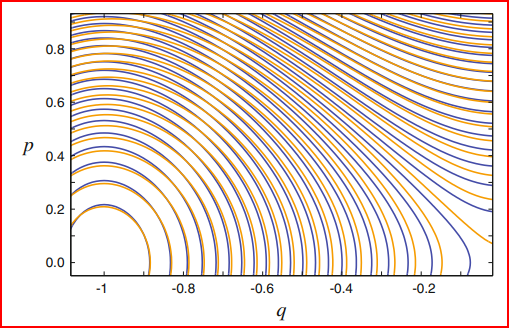
\includegraphics[scale=0.5]{img/Shadow_Hamiltonian.png}
      \end{center}
      Note that we still haven't addressed the convergence of this series, but we simply assume that the error term is bounded (which may not always be justified). Furthermore if $H_1$ and $H_2$ commute, i.e. $\{H_1, H_2\} = 0$, then there is no error in splitting. There are few special splitting cases where this would happen. An alternative approach to numerically solving the SDE is to find a scheme with Hamiltonian that has \textit{its} shadow Hamiltonian to be our target one. That is, we use a perturbed version of the original SDE and discretize it, which should lead to a higher order scheme. 

    \subsubsection{Symplectic Euler}

      Recall that splitting our Hamiltonian using 
      \begin{equation}
        H_1 = \frac{1}{2} \mathbf{p}^T \mathbf{M}^{-1} \mathbf{p}, \;\;\; H_2 = U(\mathbf{q})
      \end{equation}
      gives us the symplectic Euler method. The BCH expansion gives us the following perturbed Hamiltonian, which we can see has a leading error term of power $1$, making it a first-order scheme. 
      \begin{align*}
        \Tilde{H}_h & = H + \frac{h}{2} \{H_1, H_2\} + \frac{h^2}{12} \big( \{H_1, \{H_1, H_2\}\} - \{ H_2, \{ H_1, H_2\}\} \big) + \ldots \\
        & = H + \frac{H}{2} \nabla H_1^T \mathbf{J} \nabla H_2 + \ldots \\
        & = H + \frac{h}{2} \bigg[ \begin{pmatrix} \mathbf{0} & \mathbf{p}^T \mathbf{M}^{-1} \end{pmatrix} \begin{pmatrix} \mathbf{0} & \mathbf{I} \\ -\mathbf{I} & \mathbf{0} \end{pmatrix} \begin{pmatrix} \nabla_\mathbf{q} U(\mathbf{q}) \\ \mathbf{0} \end{pmatrix} \bigg] + \ldots \\ 
        & = H - \frac{h}{2} \mathbf{p}^T \mathbf{M}^{-1} \nabla U(\mathbf{q}) + \frac{h^2}{12} \big[ \mathbf{p}^T \mathbf{M}^{-1} U^{\prime\prime} \mathbf{M}^{-1} \mathbf{p} + \nabla U(\mathbf{q})^T \mathbf{M}^{-1} \nabla U(\mathbf{q}) \big] \\
        & - \frac{h^3}{12} \nabla U (\mathbf{q})^T \mathbf{M}^{-1} U^{\prime\prime} (\mathbf{q}) \mathbf{M}^{-1} \mathbf{p} + \mathcal{O}(h^4)
      \end{align*}

    \subsubsection{Velocity Verlet}

      Given a Hamiltonian symmetrically split into three parts
      \begin{equation}
        H(\mathbf{q}, \mathbf{p}) =  H_1 + H_2 + H_3 = \frac{1}{2} U(\mathbf{q}) + \frac{1}{2} T(\mathbf{p}) + \frac{1}{2} U(\mathbf{q})
      \end{equation}
      calculating the estimate $\exp{(h \mathcal{L}_H)} \approx \exp(\frac{h}{2} \mathcal{L}_{H_1})\,\exp(\frac{h}{2} \mathcal{L}_{H_2})\,\exp(\frac{h}{2} \mathcal{L}_{H_3})$ using the BCH lemma gives the following. Notice that the symmetricity of the splitting scheme allows us to cancel out the odd powered terms. 
      \begin{equation}
        \Tilde{H}_h = T + U + \frac{h^2}{12} \Big( \{ T, \{T, U\}\} - \frac{1}{2} \{U, \{U, T\}\} \Big) + \ldots
      \end{equation}
      The shadow Hamiltonian of the Velocity Verlet scheme applied to a single degree of freedom system of the form $H(q, p) = U(q) + \frac{1}{2} p^2$ then gives 
      \begin{align*}
        \Tilde{H}(q, p) & = H(q, p) + \frac{h^2}{24} \big(2 p U'' (q) p - (U^\prime (q))^2 \big) + h^4 \Big( \frac{1}{720} p^4 U''''(q) - \frac{1}{120} p^2 U'(q) U'''(q) \\
        & - \frac{1}{240} (U'(q))^2 U''(q) - \frac{1}{60} p^2 (U''(q))^2 + U'(q) U'''(q) \big) + \mathcal{O}(h^6) 
      \end{align*}
      Higher order symplectic integrators give higher order error terms (e.g. Yoshida-4, Imada-4). 
  
  \subsection{Hamiltonian Monte Carlo (HMC)}

    Hamiltonian Monte Carlo is one type of MCMC Metropolis-Hastings algorithms, with a Hamiltonian dynamics evolution simulated using a time-reversible, symplectic integrator (usually Velocity-Verlet). We first initialize our chain $\mathbf{X}_0 = (\mathbf{q}^0, \mathbf{p}^0)$ and compute the Hamiltonian $H(\mathbf{q}, \mathbf{p}) = U(\mathbf{q}) + \frac{1}{2} \mathbf{p}^T \mathbf{M}^{-1} \mathbf{p}$. Given that we have $\mathbf{X}_k = (\mathbf{q}_k, \mathbf{p}_k)$ at the end of the $k$th step, we then repeat the following steps: 
    \begin{enumerate}
        \item Fix $\mathbf{q}$ but pick $\mathbf{p}_{k+1} \sim \mathcal{N}(\mathbf{p}_k, \mathbf{\Sigma})$. 
        \item We run Velocity Verlet (or some other symplectic scheme) for some fixed number of steps $L$ of stepsize $h$, which models Hamiltonian flow to some new position $(\mathbf{q}_k^\prime, \mathbf{p}_k^\prime)$. This is our transition proposal. Note that for every step in Velocity Verlet, we must compute the gradient of the potential. In order to simulate Hamiltonian flow, this gradient must be exactly computed; our batch approximation will lead to discretized steps that is not deterministic anymore and do not fulfill our symplectic properties and energy preservation. 
        \item We accept this proposal with probability 
        \[\alpha = \min \bigg( 1, \frac{\exp \big[ -H(\mathbf{q}_k^\prime, \mathbf{p}_k^\prime) \big]}{\exp \big[ -H(\mathbf{q}_k, \mathbf{p}_k)\big]} \bigg)\]
        and assign $\mathbf{X}_{k+1} = (\mathbf{q}_{k+1}, \mathbf{p}_{k+1}) = (\mathbf{q}_k^\prime, \mathbf{p}_k^\prime)$ upon acceptance and $\mathbf{X}_{k+1} = \mathbf{X}_k$ if not. Note that in this step, we require the exact evaluations of our Hamiltonian. 
    \end{enumerate}
    Hamiltonian Monte Carlo is very useful if we could efficiently calculate the true log-posterior, but otherwise, the batch approximation will not model a Hamiltonian flow (and thus will not preserve the symplectic, time-reversibility, etc. properties), rendering HMC useless. 

    HMC is able to draw samples in high dimensions with greater efficiency than classical MCMC. Its key advantage is its ability to draw samples that are large distances apart by evolving them via Hamiltonian dynamics. The acceptance rate depends on the error accumulated along the sample trajectory (i.e. the error of the shadow Hamiltonian), and remains large even in high dimensions. However, a large step size (leading to greater error of shadow Hamiltonian), a large system, or a poorly behaved target density leads to greater numerical error and thus to lower sample acceptance, which induces heavy autocorrelation, necessitating a larger sample size and thus higher computational costs. 

    One approach to ease this burden is to exploit the structure of the numerical integrator error and instead target the density corresponding to a modified, \textit{shadow Hamiltonian}. This leads to higher sample acceptance rate, at the cost of some induced bias. This bias is usually well-quantified, and we can compensate for this induced bias. 

  \subsection{No U-Turn Sampler (NUTS)}


\section{Langevin Dynamics Inspired Samplers and Integrators}

    In addition to Hamiltonian dynamics, we can model the dynamics of molecular systems with Langevin dynamics. This model relies on the fact that a real world molecular system is unlikely to be present in a vacuum (there may be friction, jostling, etc.). There are two types of Langevin dynamics: overdamped and underdamped. The \textbf{Gibbs measure} mentioned below is an invariant distribution of this random process, similar to a stationary distribution of a Markov chain. That is, if we ran the model for an infinite amount of time, the Gibbs measure would be the density representing the probability of finding that particle at a certain location at any point in time. 
    \begin{enumerate}
      \item The overdamped Langevin equation does not rely on the momenta. 
      \begin{equation}
        \mathbf{\dot{q}} = - \nabla U(\mathbf{q}) + \sqrt{2 \beta^{-1}} \dot{W}
      \end{equation}
      Its Gibbs measure (invariant distribution) is 
      \begin{equation}
        \pi(\boldsymbol{\theta}) = \frac{1}{Z} \exp\big( - \beta U(\mathbf{q})\big), \text{ where } Z = \int \exp\big( - \beta U(\mathbf{q})\big)\; dq
      \end{equation}
      More precisely, given that the path $\mathbf{q}(t)$ at time $t$ is distributed according to (parameterized) density $\rho_t$, $\rho_t \rightarrow \frac{1}{Z} e^{-\beta U(\mathbf{q})}$ as $t \rightarrow +\infty$. 
      \item The underdamped Langevin equation can be interpreted as a Hamiltonian model, with the additional $- \gamma \mathbf{p} + \sqrt{2\gamma \beta^{-1}} \dot{W}$ term representing the interaction of the Hamiltonian system with an outside environment (called a heat bath or thermostat). 
      \begin{align*}
        \mathbf{\dot{q}} & = \mathbf{M}^{-1} \mathbf{p} \\
        \mathbf{\dot{p}} & = - \nabla U(\mathbf{q}) - \gamma \mathbf{p} + \sqrt{2\gamma \beta^{-1}} \mathbf{M}^{1/2} \dot{W}
      \end{align*}
      The $\gamma$ is the damping constant and $\beta$ is the inverse temperature. We can think of the term $-\gamma \mathbf{p}$ as the damping/dissipative term which "drags" the momentum $\mathbf{p}$ to $0$. The higher the $\gamma$, the stronger this drag. As $\gamma$ grows, the system spans from the inertial all the way to the diffusive (aka Brownian) regime. The term $\sqrt{2 \gamma \beta^{-1}} \dot{W}$ is the random term, which increases as temperature increases. It has invariant distribution 
      \begin{equation}
        \pi(\boldsymbol{q}, \boldsymbol{p}) = \frac{1}{Z} \exp\big( -\beta \big[ U(\mathbf{q}) + \frac{1}{2} |\mathbf{p}|^2\big] \big)
      \end{equation}
    \end{enumerate}
    To understand the relationship between the overdamped and underdamped Langevin equations and the physical systems that they represent, we can think of the overdamped equation as a limit of the underdamped one. As we set $\gamma \rightarrow +\infty$ (followed by an appropriate time scale), the underdamped Langevin equation would converge to the overdamped because the friction term would become very large, causing the momenta to dissipate instantaneously. Another way to describe this limit is to incorporate a mass matrix $\mathbf{M}$ into the underdamped: 
    \begin{align*}
      \mathbf{\dot{q}} & = \mathbf{M}^{-1} \mathbf{p} \\
      \mathbf{\dot{p}} & = - \nabla U(\mathbf{q}) - \gamma \mathbf{M}^{-1} \mathbf{p} + \sqrt{2\gamma \beta^{-1}} \dot{W}
    \end{align*}
    If we let $\mathbf{M} \rightarrow \mathbf{0}$, then we can see that the dissipative term $- \gamma \mathbf{M}^{-1}  \mathbf{p}$ will grow very large, which leads to convergence to the overdamped equation. 

    The overdamped Langevin equation is usually used to represent Brownian motion, similar to a random walk, in which there is no memory of the momenta from one time to another. The underdamped Langevin equation incorporates the momenta $\mathbf{p}$, and so the trajectory would be a lot smoother. 

    The underdamped equation has a lot nicer properties that allows us to sample efficiently. For example, when we have a double well potential $U(q)$ with the associated Gibbs measure, sampling from this potential with an overdamped integrator can cause problems. The overdamped integrator does not remember momentum, and so when crossing the energy barrier it tends to go over and recross back due to the random term. 
    \begin{center}
      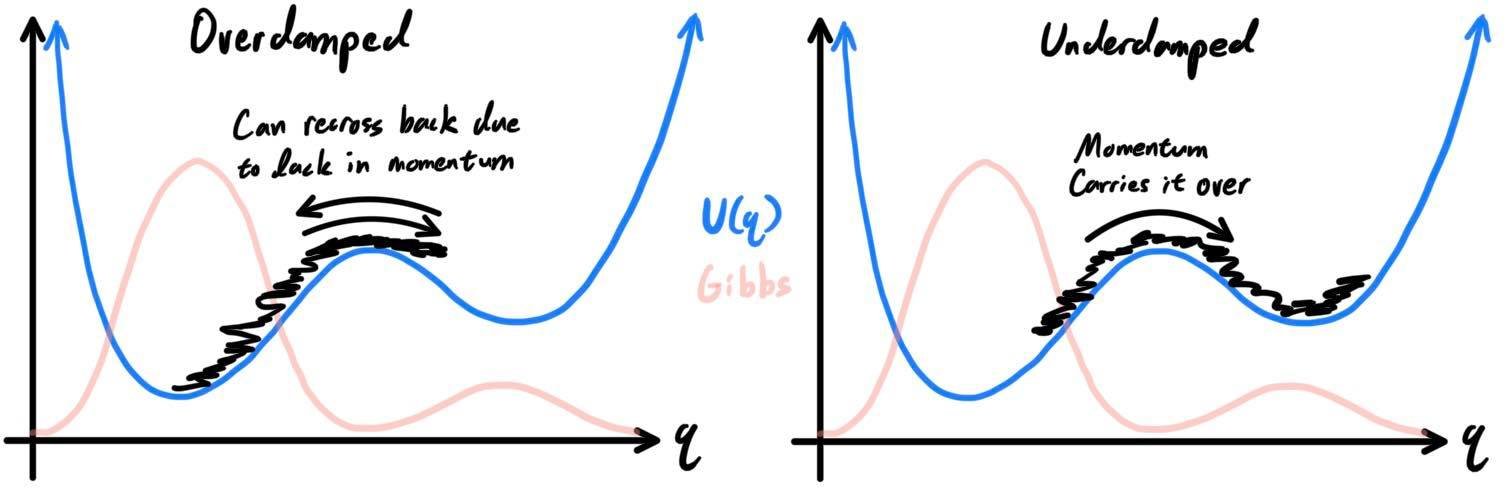
\includegraphics[scale=0.25]{img/double_well.jpg}
    \end{center}
    For the underdamped, the momentum is remembered and so when we reach over the barrier, the momentum that accelerates the particle across the well, along with the momentum that accelerates it down the well as soon as it is across, carries the particle into the other well. The choice of our friction coefficient $\gamma$ will determine how often we transition one stable state (well) to the other stable state. Choosing the right $\gamma$ is very important when sampling. 
    \begin{enumerate}
      \item If $\gamma$ is too large, we will have very similar dynamics to the overdamped Langevin equation (lots of randomness and potential recrossings), which is not ideal.
      \item If $\gamma$ is too small, it will be very similar to Hamiltonian dynamics, with a very small dissipative and random forces. It will end up just crossing back and forth smoothly and deterministically. 
    \end{enumerate}


    To compare Hamiltonian, underdamped, and overdamped dynamics, let us take a look at the phase space of the double well, with equi-Hamiltonian level sets. 
    \begin{enumerate}
      \item A Hamiltonian flow will precisely be along the level sets, since the Hamiltonian is conserved. 
      \item An underdamped Langevin flow (with $\gamma$ not too large) will move slowly between level sets. It is important not to set $\gamma$ to small since then our flow would transition very slowly between level sets and not explore our phase space very quickly. 
      \item An overdamped Langevin flow (or underdamped with large $\gamma$) will move very quickly between level sets, leading to a random walk behavior. 
    \end{enumerate}
    \begin{center}
      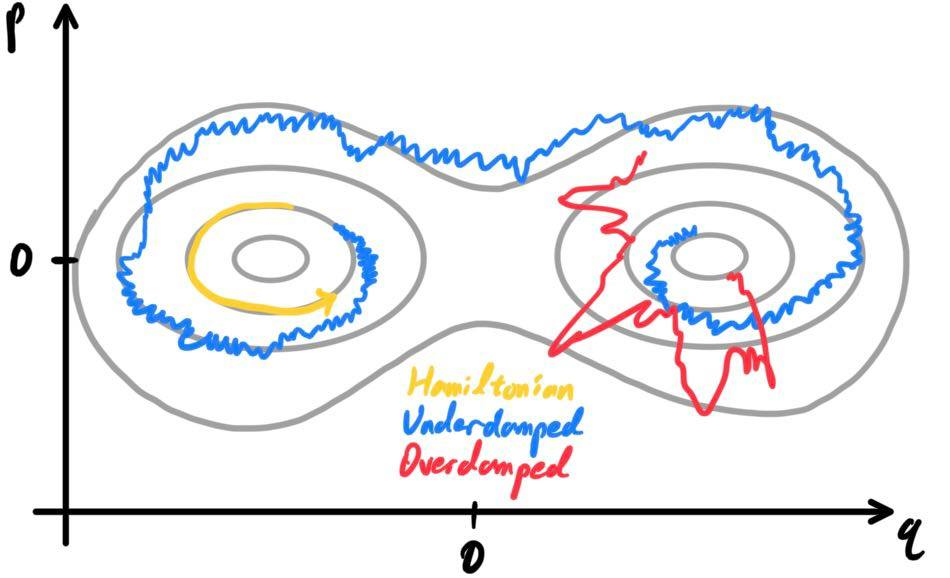
\includegraphics[scale=0.25]{img/phase_space.jpg}
    \end{center}

  \subsection{SGLD}

    Now if we add Gaussian noise to SGD, then we get \textit{Stochastic Gradient Langevin Dynamics (SGLD)} sampler, which is the discretized form of the overdamped Langevin equation 
    \begin{equation}
      \mathbf{\dot{q}} = - M^{-1} \nabla_\mathbf{q} U(\mathbf{q}) + \sqrt{2 \beta^{-1}} M^{-1/2} \dot{W}
    \end{equation}
    where $M$ is the mass matrix, $\beta$ the inverse temperature, and $\dot{W}$ a Weiner process. If the gradient computations are exact, then SGLD reduces to the \textit{Langevin Monte Carlo} algorithm. This algorithm is also a reduction of Hamiltonian Monte Carlo, consisting of a single leapfrog step proposal rather than a series of steps. Since SGLD can be formulated as a modification of both SGD and MCMC methods, it lies at the intersection between optimization and sampling algorithms. The method maintains SGD's ability to quickly converge to regions of low cost while providing samples to facilitate posterior inference. 

    If we set the mass matrix to be $I$, we can update $\mathbf{q}$ according to the following discretization. 
    \begin{equation}
      \mathbf{q}_{t+1} = \mathbf{q}_t - \nabla_{\mathbf{q}} U(\mathbf{q}_t) + \sqrt{2 \beta^{-1}} \, \boldsymbol{\epsilon}, \;\;\;\;\; \boldsymbol{\epsilon} \sim \mathcal{N}(\mathbf{0}, \mathbf{I})
    \end{equation}

    \begin{algorithm}
      \caption{SGLD}\label{alg:sgld}
      \begin{algorithmic}

      \Require Initial $\boldsymbol{\theta}_0$, Stepsize function $h(t)$, Minibatch size $m$

      \For{$t = 0$ to $T$}
          \State $\hat{g}(\theta_t) \gets \nabla_\theta \log{p(\theta_t \mid M_m(\mathcal{D}))}$
          \State $\epsilon_t \sim \mathcal{N}(0, I)$
          \State $\theta_{t+1} \gets \theta_t + h(t) \cdot \hat{g}(\theta_t) + \sqrt{2 h(t) \beta^{-1}} \, \epsilon_t$
      \EndFor

      \end{algorithmic}
    \end{algorithm}

    We can incorporate the mass matrix, which is approximated by the precision of the log posterior ($M^{-1} = \Sigma$), for adapting (along with preconditioning if needed). This would result in the discretized step: 
    \begin{equation}
      \mathbf{q}_{t+1} = \mathbf{q}_t - M^{-1} \nabla_{\mathbf{q}} U(\mathbf{q}_t) + \sqrt{2 \beta^{-1}} M^{-1} \, \boldsymbol{\epsilon}
    \end{equation}

    \begin{algorithm}
      \caption{Adaptive SGLD}\label{alg:adaptive_sgld}
      \begin{algorithmic}

      \Require Initial $\boldsymbol{\theta}_0$, Stepsize function $h(t)$, Minibatch size $m$, Adaptation burn-in $B$, Adaptation frequency $U$
      \State $\mu_0^{\mathrm{emp}} \gets 0$
      \State $\Sigma_0 \gets I$
      \State $\Sigma_0^{\mathrm{emp}} \gets I$

      \For{$t = 0$ to $T$}
          \State $\hat{g}(\theta_t) \gets \nabla_\theta \log{p(\theta_t \mid M_m(\mathcal{D}))}$
          \State $\epsilon_t \sim \mathcal{N}(0, \Sigma^t)$
          \State $\theta_{t+1} \gets \theta_t + h(t) \, \Sigma_t \, \hat{g}(\theta_t) + \sqrt{2 h(t) \beta^{-1}} \, \epsilon_t$
          
          \State $\Sigma^\mathrm{emp}_{t+1} \gets \frac{1}{t+1} \big[(\theta^{t+1} - \mu_t) (\theta^{t+1} - \mu_t)^T - \Sigma^\mathrm{emp}_t \big]$
          \State $\mu_{t+1}^\mathrm{emp} \gets \mu_t + \frac{1}{t+1} [ \theta_{t+1} - \mu_t ]$
          
          \If{$t > B$ and $t$ is divisible by $U$}
              \State $\Sigma_{t+1} \gets \Sigma_{t+1}^{\mathrm{emp}}$
          \EndIf
      \EndFor

      \end{algorithmic}
    \end{algorithm}

  \subsection{MALA}

    We can slightly modify SGLD to get the \textit{Metropolis Adjusted Langevin Algorithm (MALA)} sampler, which has two differences from SGLD: 
    \begin{enumerate}
      \item SGLD uses a minibatch approximation of the gradient (hence the name stochastic), while MALA always uses the entire dataset.
      \item MALA has an additional Metropolis accept/reject step on the proposal state, while SGLD always "accepts" the new state.
    \end{enumerate}
    For the sake of conciseness, we will provide the adaptive MALA algorithm. 

    \begin{algorithm}
      \caption{Adaptive MALA}\label{alg:adaptive_mala}
      \begin{algorithmic}

      \Require Initial $\boldsymbol{\theta}_0$, Stepsize function $h(t)$, Minibatch size $m$, Adaptation burn-in $B$, Adaptation frequency $U$
      \State $\mu_0^{\mathrm{emp}} \gets 0$
      \State $\Sigma_0 \gets I$
      \State $\Sigma_0^{\mathrm{emp}} \gets I$

      \For{$t = 0$ to $T$}
          \State $\hat{g}(\theta_t) \gets \nabla_\theta \log{p(\theta_t \mid \mathcal{D})}$
          \State $\epsilon_t \sim \mathcal{N}(0, \Sigma^t)$
          \State $P_{t+1} \gets \theta_t + h(t) \, \Sigma_t \, \hat{g}(\theta_t) + \sqrt{2 h(t) \beta^{-1}} \, \epsilon_t$ 
          
          \If{$\log{p(P_{t+1} \mid \mathcal{D})} \geq \log{p(\theta_t \mid \mathcal{D})}$} 
              \State $\theta_{t+1} \gets P_{t+1}$
          \Else 
              \State $\delta \sim \mathrm{Uniform}[0, 1]$ 
              \If{$\delta < \log{p(P_{t+1} \mid \mathcal{D})} / \log{p(\theta_t \mid \mathcal{D})}$}
                  \State $\theta_{t+1} \gets P_{t+1}$ 
              \Else 
                  \State $\theta_{t+1} \gets \theta_t$
              \EndIf
          \EndIf
          
          \State $\Sigma^\mathrm{emp}_{t+1} \gets \frac{1}{t+1} \big[(\theta^{t+1} - \mu_t) (\theta^{t+1} - \mu_t)^T - \Sigma^\mathrm{emp}_t \big]$
          \State $\mu_{t+1}^\mathrm{emp} \gets \mu_t + \frac{1}{t+1} [ \theta_{t+1} - \mu_t ]$
          
          \If{$t > B$ and $t$ is divisible by $U$}
              \State $\Sigma_{t+1} \gets \Sigma_{t+1}^{\mathrm{emp}}$
          \EndIf
      \EndFor

      \end{algorithmic}
    \end{algorithm}

  \subsection{Langevin Numerical Integrators}

    \subsubsection{Euler-Mayurama Method}

      The Euler-Mayurama integrator models Brownian dynamics/overdamped Langevin dynamics. We update the position vector $\mathbf{q}$ with a single timestep: 
      \begin{equation}
        \mathbf{q}_{k+1} = \mathbf{q}_k + h \mathbf{M}^{-1} \nabla U(\mathbf{q}_k) + \sqrt{2 h k_B T} \mathbf{M}^{-1/2} \mathbf{R}_k
      \end{equation}
      where $\mathbf{R}_k$ are vectors of standard independent Gaussian $\mathcal{N}(0, I)$ variables, resampled at each step. Since $k_B$ is the Boltzmann constant, we can set $\beta = (k_B T)^{-1}$ to be the \textbf{inverse temperature} parameter, reducing the above to 
      \begin{equation}
        \mathbf{q}_{k+1} = \mathbf{q}_k + h \mathbf{M}^{-1} \nabla U(\mathbf{q}_k) + \sqrt{2 h \beta^{-1}} \mathbf{M}^{-1/2} \mathbf{R}_k
      \end{equation}
      This EM discretized scheme has an invariant measure $\hat{\pi}_h$ that is also an approximation of the true Gibbs measure $\pi$ of the original Langevin equation. We subscript it with the step size $h$ since convergence will be dependent on $h$. 
      \begin{equation}
        \hat{\pi}_h (\mathbf{q}) = \pi(\mathbf{q}) + \mathcal{O}(h)
      \end{equation}
      We can interpret the $\mathcal{O}(h)$ term as a term $\rho(\mathbf{q}) h$ (where $\rho$ is some density) that vanishes linearly as $h \rightarrow 0$. 

    \subsubsection{Leimkuhler-Matthews Method}

      The Leimkuhler-Matthews method also finds discretized solutions to Brownian dynamics, with position update of 
      \begin{equation}
        \mathbf{q}_{k+1} = \mathbf{q}_k + h \mathbf{M}^{-1} \nabla U(\mathbf{q}_k) + \sqrt{2 h \beta^{-1}} \mathbf{M}^{-1/2} \bigg( \frac{\mathbf{R}_k + \mathbf{R}_{k-1}}{2} \bigg)
      \end{equation}

    \subsubsection{BAOAB Method}

      The BAOAB method is a symplectic integrator that models an undampened Langevin flow, with the following steps per timestep: 
      \begin{align*}
        \mathbf{p}_{k + 1/2} & = \mathbf{p}_k - \frac{h}{2} \nabla U(\mathbf{q}_k) \\
        \mathbf{q}_{k + 1/2} & = \mathbf{q}_k + \frac{h}{2} \mathbf{M}^{-1} \mathbf{p}_{k + 1/2} \\
        \mathbf{\hat{p}}_{k + 1/2} & = e^{-h \gamma} \mathbf{p}_{k + 1/2} + \sqrt{\beta^{-1} (1 - e^{-2\gamma h})} \mathbf{M}^{1/2} \mathbf{R}_k \\ 
        \mathbf{q}_{k + 1} & = \mathbf{q}_{k + 1/2} + \frac{h}{2} \mathbf{M}^{-1} \mathbf{\hat{p}}_{k + 1/2} \\
        \mathbf{p}_{k + 1} & = \mathbf{\hat{p}}_{k + 1/2} - \frac{h}{2} \nabla U(\mathbf{q}_{k + 1}) 
      \end{align*}
      where $\mathbf{R}_k$ are vectors of standard independent Gaussian $\mathcal{N}(0, I)$ variables, resampled at each step. Notice that the O step incorporates the randomness within this integrator. 
      BAOAB is a discretization of an underdamped Langevin flow, but BAOAB with an extremely large $\gamma$ would be similar to a discretization of an overdamped Langevin flow. There are other BAO splitting schemes, such as OBABO, OABAO, and ABOBA, but BAOAB is the best. 

      Recall that the true invariant measure of underdamped Langevin equations is $\pi(\mathbf{q}, \mathbf{p}) = \frac{1}{Z} \exp \big( -U(\mathbf{q}) + \frac{1}{2} |\mathbf{p}|^2 \big)$. BAOAB is a second-order scheme, meaning that the invariant measure $\hat{\pi}_h$ of this discretized scheme is a second order approximation of $\pi$. With some analysis, we can see that $\hat{\pi}$ is of order 2 (in fact, the BAO methods are all of order 2). 
      \begin{align*}
        \hat{\pi}_h (\mathbf{q}, \mathbf{p}) & = \pi(\mathbf{q}, \mathbf{p}) + C h^2 f_2 (\mathbf{q}, \mathbf{p}) \pi(\mathbf{q}, \mathbf{p}) + \mathcal{O}(h^4) \\
        & = \pi(\mathbf{q}, \mathbf{p}) + \mathcal{O}(h^2)
      \end{align*}
      where $f_2$ is some function such that $\mathbb{E}_\mathbf{p} [f_2] = 0$. But we are typically interested in just $\mathbf{q}$ when looking at the Gibbs density of a system, so we look at the marginal measure of $\mathbf{q}$: $\hat{\pi}_h (\mathbf{q}) = \int_\mathbf{p} \hat{\pi}_h (\mathbf{q}, \mathbf{p})\, d\mathbf{p}$, leading us to rewrite the above as
      \begin{equation}
        \hat{\pi}_h (\mathbf{q}) = \pi(\mathbf{q}) + C h^2 f_2 (\mathbf{q}) \pi(\mathbf{q}) + \mathcal{O}(h^4)
      \end{equation}
      Furthermore, the constant $C \in \mathcal{O}(1/ \gamma)$, where $\gamma$ is the friction constant seen in the underdamped Langevin equation. This means that as $\gamma$ increases, $C$ decreases, and so for sufficiently big $\gamma$, the second term vanishes and we have an order 4 approximation. Depending on what specific scheme (BAOAB, ABOBA, etc.), the constant $C$ would be different. Therefore, the BAOAB scheme is of order 2 in underdamped dynamics and of order 4 in overdamped dynamics. 

  \subsection{Splitting Methods for Langevin Dynamics}

    Just like how to split Hamiltonians into components to build symplectic integrators, we can split an SDE (specifically, the undamped Langevin equations) as such 
    \begin{equation}
      \begin{pmatrix} \mathbf{\dot{q}} \\ \mathbf{\dot{p}} \end{pmatrix} = \underbrace{\begin{pmatrix} \mathbf{M}^{-1} \mathbf{p} \\ \mathbf{0} \end{pmatrix}}_{A} + \underbrace{\begin{pmatrix} \mathbf{0} \\ -\nabla U(\mathbf{q}) \end{pmatrix}}_{B} + \underbrace{\begin{pmatrix} \mathbf{0} \\ -\gamma \mathbf{p} + \sqrt{2 \gamma \beta^{-1}} \mathbf{M}^{1/2} \dot{W} \end{pmatrix}}_{O}
    \end{equation}
    where each of the three parts $A, B, O$ may be solved exactly with discretizations given as 
    \begin{align*}
      \hat{\Phi}_h^A (\mathbf{q}_k, \mathbf{p}_k) & = \big(\mathbf{q}_k + h \mathbf{M}^{-1} \mathbf{p}_k, \mathbf{p}_k \big) \\
      \hat{\Phi}_h^B (\mathbf{q}_k, \mathbf{p}_k) & = \big(\mathbf{q}_k, \mathbf{p}_k - h \nabla U(\mathbf{q}_k) \big) \\
      \hat{\Phi}_h^O (\mathbf{q}_k, \mathbf{p}_k) & = \big(\mathbf{q}_k, e^{-\gamma h} \mathbf{p}_k + \sqrt{\beta^{-1} (1 - e^{-2 \gamma h})} \mathbf{M}^{1/2} \mathbf{R}\big)
    \end{align*}
    and therefore, composing them with each other gives specific schemes. For example, the ABO scheme is 
    \begin{equation}
      \hat{\Phi}_h^{[ABO]} = \hat{\Phi}_h^O \circ \hat{\Phi}_h^B \circ \hat{\Phi}_h^A
    \end{equation}
    We can also symmetrically split these steps down further (must it be symmetric? since we don't have to worry about order of shadow Hamiltonian). For example, 
    \begin{align*}
      \hat{\Phi}_h^{[BABO]} & = \hat{\Phi}_h^O \circ \hat{\Phi}_{h/2}^B \circ \hat{\Phi}_h^A \circ \hat{\Phi}_{h/2}^B \\
      \hat{\Phi}_h^{[BAOAB]} & = \hat{\Phi}_{h/2}^B \circ \hat{\Phi}_{h/2}^A \circ \hat{\Phi}_h^O \circ \hat{\Phi}_{h/2}^A \circ \hat{\Phi}_{h/2}^B
    \end{align*}
    There are much more Langevin integrators that we can construct from the A, B, O blocks. 


\section{Simulated Annealing}

  Unlike the previous optimizers, \textit{simulated annealing} is useful in finding \textit{global} optima in the presence of multimodal functions within a usually very large discrete space $\mathcal{S}$. Given some function $f$ defined on $\mathcal{S}$, we would like to find its global maximum. Rather than picking the "best move" using gradient information (like SGD), we propose a random move. Let us start at a state $\theta_k$ and propose a random $P_{k+1}$. We denote $\Delta f = f(P_{k+1}) - f(\theta_k)$. 
  \begin{enumerate}
      \item If the selected move improves the solution (i.e. $\Delta f \geq 0$, then it is always accepted and we set $\theta_{k+1} \gets P_{k+1}$. 
      \item Otherwise, when $\Delta f < 0$ it makes the move with the following acceptance probability 
      \[p(\theta_{k+1} \gets P_{k+1} \mid \Delta f < 0) = e^{\Delta f / T(t)}\]
  \end{enumerate}
  We can see that if $\Delta f$ is very negative (the move is very bad), then this probability of acceptance decreases as well. Furthermore, $T(t)$ represents some sort of "temperature" that we anneal as a function of time, called the \textit{annealing schedule}. $T$ starts off at a high value, increasing the rate at which bad moves are accepted, which promotes exploration of $\mathcal{S}$ and allows the algorithm to travel to suboptimal areas. As $T$ decreases, the vast majority of steps move uphill, promoting exploitation, which means that once the algorithm is in the right search space, there is no need to search other sections of the search space. 

  \begin{algorithm}
  \caption{Simulated Annealing}\label{alg:sim_anneal}
  \begin{algorithmic}

  \Require Initial $\theta_0$, Transition kernel $\pi(\theta_{k+1} \mid \theta_k)$, Annealing schedule $T(t)$

  \For{$t = 0$ to $T$ until convergence}
      \State $P_{t+1} \sim \pi( \cdot \mid \theta_t)$
      
      \If{$f(P_{t+1}) - f(\theta_t) \geq 0$} 
          \State $\theta_{t+1} \gets P_{t+1}$ 
      \Else 
          \State $\delta \sim \mathrm{Uniform}[0, 1]$
          \If{$\delta < \exp[(f(P_{t+1}) - f(\theta_t))/T(t)]$}
              \State $\theta_{t+1} \gets P_{t+1}$ 
          \Else 
              \State $\theta_{t+1} \gets \theta_t$ 
          \EndIf
      \EndIf
  \EndFor

  \end{algorithmic}
  \end{algorithm}

  This algorithm is very easy to implement and provides optimal solutions to a wide range of problems (e.g. TSP and nonlinear optimization), but it can take a long time to run if the annealing schedule is very long. We can stop either if $T$ reaches a certain threshold or if we have determined convergence. 



\bibliography{./bibfile}
\bibliographystyle{alpha}

\end{document}
